\documentclass{scrreprt}
\KOMAoptions{parskip=half*}
\usepackage{mathtools}
\numberwithin{equation}{chapter}
\usepackage{graphicx}
\usepackage{hyperref}
\hypersetup{
  colorlinks=true,
  linkcolor=gray,
  urlcolor=purple
}
\usepackage[chapter,newfloat=true]{minted}
\usemintedstyle[cpp]{autumn}
\newminted[cpp]{cpp}{bgcolor=bgc}

\begin{document}
\definecolor{bgc}{rgb}{0.95,0.98,0.95}
\title{ThinkChess\textsuperscript{++}}
\author{Oliver Krischer}
\subtitle{Build a chess app with C\textsuperscript{++} and learn to play along the way.}
\maketitle
\begin{abstract}
  If you have ever wondered how to program a simple chess app for yourself,
  this tutorial is the right starting point.
  We are going to explore the machanics of the game, how to maintain and display the game status,
  and how to find a good next move.

  To that goal we we'll also dive into data structures (\emph{lists, trees, graphs}),
  and explore some basic search algorithms based on these data structures.

  After working through this tutorial, you will not only have a running chess app,
  but also will be proficient in playing chess at an amateur level. 

  The souce code of the program and the documentation is available at
  \href{https://github.com/okrischer/ThinkChess}{github}.
\end{abstract}
\tableofcontents

\chapter{Display the Game}

I've chosen the \emph{Simple and Fast Multimedia Library}
\href{https://www.sfml-dev.org/index.php}{SFML} for creating the graphical user interface
of the app.
It lives up to its name and is available on all major platforms and programming languages.

In this chapter we'll learn how to display the board and the chess pieces on it.
In order to show valid moves for each piece, we will also learn the basic rules of the game.

I'm using \href{https://cmake.org/}{CMake} for building the C\textsuperscript{++} code,
and the SFML CMake project template, which will build the SFML libraries.
So you will need to have the following components installed on your machine:

\begin{itemize}
  \item a decent C\textsuperscript{++} compiler (any of the major compilers will do)
  \item the \emph{git} tool
  \item the \emph{cmake} tool
  \item the required system packages for
    \href{https://www.sfml-dev.org/tutorials/2.6/start-cmake.php}{SFML}
\end{itemize}
 
On a linux system, all those components can be installed with your systems package manager
(e.g. with \texttt{apt-get} on Ubuntu).
For Mac OS, just use the included \texttt{clang++} compiler and install
missing components with \href{https://brew.sh/}{homebrew}:
\texttt{<brew install git cmake sfml>}.

When everything is in place, just clone my repository with\\
\texttt{<git clone https://github.com/okrischer/ThinkChess.git>}\\
and execute \texttt{<cmake -B build>} from the root folder of your local copy.\\
If everything went well, change to the \texttt{build} folder and execute \texttt{<cmake --build .>}.\\
Voila, you have a simple chess app, which you can start with \texttt{<./ThinkChess>}.

I strongly encourage you to code all the following steps with an editor of your choice
for yourself and see if you can get the code running. Nothing is gained if you just skim
over the provided source code.

If you have \LaTeX\ installed on your machine, you can also build the documentation
with \texttt{<pdflatex -shell-escape ThinkChess++.tex>} from the \texttt{doc} folder,
which will produce this document.

\section{Displaying the board and the pieces}

Let's start with the basic framework for displaying something with SFML:

\begin{cpp*}{linenos}
#include <SFML/Graphics.hpp>

int main() {
  sf::ContextSettings settings;
  settings.antialiasingLevel = 8;
  auto window = sf::RenderWindow{ {640u, 640u}, "ThinkChess++",
              sf::Style::Default, settings };
  window.setFramerateLimit(10);

  while (window.isOpen()) {
    for (auto event = sf::Event{}; window.pollEvent(event);) {
      if (event.type == sf::Event::Closed) {
        window.close();
      }
    }
    window.draw(bs);
    window.display();
  }
}
\end{cpp*}

This is the main file for our app (\texttt{app/main.cpp}).
Thus, it defines the \mintinline{cpp}{int main()} function (3) as the starting point of the app.
The numbers in paranthesis \texttt{(x)} always refer to the last code snippet.\\
In order to access SFML functionality, we have to \mintinline{cpp}{#include} the SFML Graphics
library (1), which was built by \emph{cmake}.\\
First, we define the context (4) and set the antialiasing level to 8 within the context (5).\\
Next, we define the main window for our app (6), setting its size, title, style, and the context
settings.\\
Then we set the framerate to 10 (8), i.e. 10 frames per second; we don't need more
for such a static app, and the app will keep responsive with that.\\
Next comes the central part: entering the main game loop (10-18). The game loop usually contains
three steps:

\begin{enumerate}
  \item an event loop, processing all user inputs for the current frame (11-15)
  \item several drawing instructions (16) for all items to appear in the frame
  \item a call to \mintinline{cpp}{window.display()}, which causes all drawn elements to be
    actually displayed.
\end{enumerate}

\subsection{The board}
We don't have anything to draw yet; let's change this by adding a chessboard
within the main function, just before entering the game loop:

\begin{cpp*}{linenos}
  sf::Texture bi;
  bi.loadFromFile("../img/chessboard.jpg");
  sf::Sprite bs;
  bs.setTexture(bi);
\end{cpp*}

Here, we create a SFML texture (1) and load an image from the file system into that texture (2).
Then we create a SFML sprite (3) and set its texture  to that image (4).

If you run the app now, you would see an empty chess board:

\begin{center}
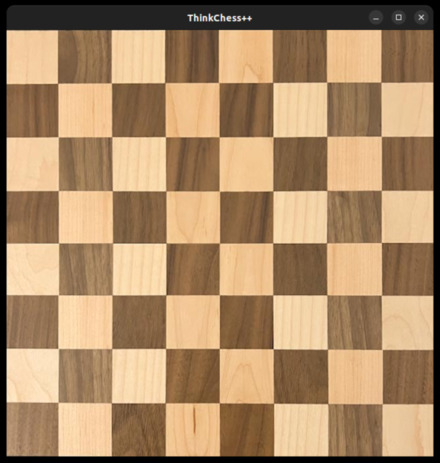
\includegraphics[width=.5\linewidth]{img/emptyBoard.jpg}
\end{center}

\subsection{The pieces}
Not that interesting so far, so we're going to add the chess pieces at their initial position.
For that, let's introduce the pieces at first: they come in two colors, \emph{white}
and \emph{black}, each for one player, and they are called as follows
(from left to right in the image below):

\begin{center}
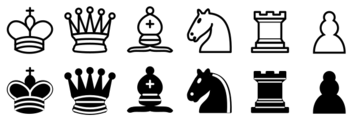
\includegraphics[width=.5\linewidth]{../img/figures.png}
\end{center}

\begin{center}
\begin{tabular}{l | c | c | c | c | c | c}
  \hline
  Piece & King & Queen & Bishop & Knight & Rook & Pawn \\
  quantity & 1 & 1 & 2 & 2 & 2 & 8 \\
  value  & - & 8 & 3 & 3 & 4 & 1 \\
  \hline
\end{tabular}
\end{center}

Every piece, except the king, has a value assigned to it; this is just by convention and
not necessary for the original game play.
The value indicates the strength of the piece and serves for a basic evaluation of each players
position during the game.

The \emph{Queen} is the most powerful piece in the game, followed by the \emph{Rook};
those two are also called \emph{major pieces}.
Then we have the \emph{Bishop} and the \emph{Knight}, both of equal value, building the
group of \emph{minor pieces}.
The least worthy piece is the \emph{Pawn}.

But why has the \emph{King} no value assigned?\\
The goal of the game is to put your opponents \emph{King} in a position, where it is attacked
by any of your own pieces (an attack is the threat to capture a piece with the next move).
We call this position \emph{check}.\\
If a player cannot respond to a \emph{check} in the very next move (i.e. defend his \emph{King}),
the game is over, and that player has lost the game.
We call this position \emph{checkmate}.\\
Thus, the \emph{King} is never actually captured, it stays on the board until the end of the game.
With that, it doesn't make any sense to give it a value for evaluating a players position. 

We'll cover the movement of the pieces in great detail in the next section~\ref{subsec:validmoves}.
But, for now, let's concentrate on how to display the pieces:

\begin{cpp*}{linenos}
  sf::Texture figures;
  figures.loadFromFile("../img/figures.png");

  sf::Sprite wk;
  wk.setTexture(figures);
  wk.setTextureRect(sf::IntRect(0,0,60,60));

  sf::Sprite bk;
  bk.setTexture(figures);
  bk.setTextureRect(sf::IntRect(0,60,60,60));
  // --- snip ---
\end{cpp*}

We have loaded a texture, containing the figures of all pieces (2).
Then we define distinct sprites for every piece, calling them \emph{wk} for the white king (4),
\emph{bk} for the black king (8), and so forth.\\
Finally, we cut out the matching parts of the \mintinline{cpp}{figures} texture and assign
them to every distinct sprite (6, 10).


Notice, that I've taken care that all the sprites have the same size of
$60 \times 60$ pixels.
As the board has a size of $640 \times 640$ pixels, containing $8 \times 8$ light and dark squares,
every square on the board has a size of $80 \times 80$ pixels.
That allows us to place the sprites evenly on the board with an offeset of 10 pixels to the
boundary of each square.

\subsection{Keeping track of the pieces}
In order to actually place the pieces on the board, we need a data structure, being able to
keep track of the 64 squares.
As it turns out, an $8 \times 8$ vector matrix is a good fit for that:

\begin{cpp}
vector<vector<Piece*>> board(8, vector<Piece*>(8));
\end{cpp}

You could have used any type of vector matrix for keeping track of the pieces,
but I've chosen an \emph{object-oriented} approach:
every piece is represented by a raw pointer (indicated with the *) to an instance of the type
\mintinline{cpp}{Piece}.
That allows for greater flexibility implementing the game logic: instead of putting
the logic for the pieces in the main file, we are going to implement it in a new file
\texttt{app/pieces.cpp}.

So, let's have a look on how \mintinline{cpp}{Piece} is actually implemented:

\begin{cpp}
#pragma once
#include <vector>

// public interface for pieces
class Piece {
public:
  virtual ~Piece() {}
  virtual char getType() = 0;
  virtual char getValue() = 0;
  virtual bool isWhite() = 0;
  virtual bool isCaptured() = 0;
  virtual int getRow() = 0;
  virtual int getCol() = 0;
  virtual void capture() = 0;
  virtual bool isValid(std::vector<std::vector<Piece*>>& bd,
                       int r, int c) = 0;
};
\end{cpp}

As you may have guessed, this code snippet is not from the \texttt{pieces.cpp} file, but from its
\emph{header} file, located at \texttt{include/pieces.hpp}.
I've decided to separate the compilation units into a public interface (the header file) and
an implementation file.
That allows to use the definitions of the header file in any other implementation file and
gives us even more flexibility in structuring the source code.

\mintinline{cpp}{Piece} is declared as a pure \emph{abstract} interface.
That means, it doesn't have a \emph{constructor}, and all the member functions are marked
as \mintinline{cpp}{virtual}.
Thus, you cannot instanciate it directly, and to make any use of it, we have to create
\emph{derived} classes (subclasses of \mintinline{cpp}{Piece}) for every piece, which will
implement the virtual functions.
The reason for doing so is: we need different implementations for performing moves for
each piece, but also a common type for storing them in the board matrix. 

The concrete types for \mintinline{cpp}{Piece} are implemented like so:

\begin{cpp*}{linenos}
class King : public Piece {
public:
  ~King() {}
  King(bool w, int r, int c) : type{'K'}, white{w}, value{0},
                              captured{false}, row{r}, col{c} {}

  char getType() override { return type; }
  char getValue() override { return value; }
  bool isWhite() override { return white; }
  bool isCaptured() override { return captured; }
  int getRow() override { return row; }
  int getCol() override { return col; }
  bool isValid(std::vector<std::vector<Piece*>>& bd, int r, int c)
    override;

private:
  char type;
  bool white;
  short value;
  bool captured;
  int row;
  int col;
};
\end{cpp*}

The other pieces are implemented likewise; the only difference between them so far is the
implementation of the member function \mintinline{cpp}{isValid} (13).
I decided to leave all the class definitions in the header file, and moved only the
implementation for \mintinline{cpp}{isValid} to the file \texttt{app/pieces.cpp}.
We'll study these implementations in the next section~\ref{subsec:validmoves}.

For now, we are only interested in the type definitions:\\
each of them is derived from \mintinline{cpp}{class Piece} (1) and has a \emph{destructor} (3),
which will be called by the compiler when an instance of the class is destroyed.
This will happen automatically, whenever an \emph{automatic} variable gets out of scope.
But, if a reference to an instance was created explicitly (using the keyword \mintinline{cpp}{new}),
we have to \mintinline{cpp}{delete} that object explicitly in order to avoid \emph{memory leaks}.

Next, we have the \emph{constructor} (4-5):\\
it initializes a new instance with its type (which we need only for drawing the correct sprite),
the color of the piece (white or black), its value, and the current position
of the piece (the row and column of the piece in the board matrix).

The following member functions (7-12) are just \emph{getters} to retrieve the
\mintinline{cpp}{private} member types.

With the derived \mintinline{cpp}{Piece} types in place, we can initially fill the board matrix:

\begin{cpp}
void reset_board(vector<vector<Piece*>>& bd) {
  for (auto rank : bd) {
    for (auto piece : rank) {
      delete piece;
    }
  }
  // rank 8 (black)
  bd[0][0] = new Rook(0,0,0);
  bd[0][1] = new Knight(0,0,1);
  bd[0][2] = new Bishop(0,0,2);
  bd[0][3] = new Queen(0,0,3);
  bd[0][4] = new King(0,0,4);
  bd[0][5] = new Bishop(0,0,5);
  bd[0][6] = new Knight(0,0,6);
  bd[0][7] = new Rook(0,0,7);
  // rank 7 (black)
  bd[1][0] = new Pawn(0,1,0);
  bd[1][1] = new Pawn(0,1,1);
  bd[1][2] = new Pawn(0,1,2);
  bd[1][3] = new Pawn(0,1,3);
  bd[1][4] = new Pawn(0,1,4);
  bd[1][5] = new Pawn(0,1,5);
  bd[1][6] = new Pawn(0,1,6);
  bd[1][7] = new Pawn(0,1,7);
  // rank 2 (white)
  bd[6][0] = new Pawn(1,6,0);
  bd[6][1] = new Pawn(1,6,1);
  bd[6][2] = new Pawn(1,6,2);
  bd[6][3] = new Pawn(1,6,3);
  bd[6][4] = new Pawn(1,6,4);
  bd[6][5] = new Pawn(1,6,5);
  bd[6][6] = new Pawn(1,6,6);
  bd[6][7] = new Pawn(1,6,7);
  // rank 1 (white)
  bd[7][0] = new Rook(1,7,0);
  bd[7][1] = new Knight(1,7,1);
  bd[7][2] = new Bishop(1,7,2);
  bd[7][3] = new Queen(1,7,3);
  bd[7][4] = new King(1,7,4);
  bd[7][5] = new Bishop(1,7,5);
  bd[7][6] = new Knight(1,7,6);
  bd[7][7] = new Rook(1,7,7);
}
\end{cpp}

That seems tedious, but thankfully we have to do this only once.
I've placed the initialization code within a function \mintinline{cpp}{void reset_board()},
just in case we want to reset the board later (e.g. when starting a new game).
The board is passed as an automatic reference to the function (indicated by the \& after the
parameter type), such that we are able to modify the board directly,
instead of working with a copy of the board.

The code in the first three lines actually resets the board by deleting all existing
references to pieces.
When setting the pieces, you have to be careful: every piece must be initialized with exactly the
same coordinates from the board (and of course with the correct color: 0 for black and 1 for white).

The rows of a chessboard are called \emph{ranks}, while the colums are called
\emph{files}.
The ranks are indicated by the numbers 1 to 8, whereas the files are indicated by the letters
\texttt{a} to \texttt{h}, both starting at the lower left square (the dark field \texttt{a1}):
\begin{samepage}
\begin{verbatim}
8 . . . . . . . .
7 . . . . . . . .
6 . . . . . . . .
5 . . . . . . . .
4 . . . . . . . .
3 . . . . . . . .
2 . . . . . . . .
1 . . . . . . . .
  a b c d e f g h
\end{verbatim}

With the initialization code above, the pieces will be placed like so on the board:

\begin{verbatim}
8 R N B Q K B N R
7 P P P P P P P P
6 . . . . . . . .
5 . . . . . . . .
4 . . . . . . . .
3 . . . . . . . .
2 P P P P P P P P
1 R N B Q K B N R
  a b c d e f g h
\end{verbatim}
\end{samepage}

Observe that we abbreviate the \emph{Knight} with the letter \texttt{N} to avoid confusion with
the \emph{King}.
So, the white \emph{Queen} is placed at \texttt{d1}, the black \emph{Queen} at \texttt{d8},
and so forth.

\subsection{Drawing the pieces}
Now we can use the filled board matrix to actually draw the pieces within the game loop of the
main function:

\begin{cpp*}{linenos}
    // draw board
    window.draw(bs);
    // draw pieces
    for (int row = 0; row < 8; row++) {
      for (int col = 0; col < 8; col++) {
        if (board[row][col]) {
          auto piece = board[row][col];
          sf::Sprite pc;
          switch (piece->getType()) {
          case 'K':
            piece->isWhite() ? pc = wk : pc = bk;
            break;
          case 'Q':
            piece->isWhite() ? pc = wq : pc = bq;
            break;
          case 'R':
            piece->isWhite() ? pc = wr : pc = br;
            break;
          case 'B':
            piece->isWhite() ? pc = wb : pc = bb;
            break;
          case 'N':
            piece->isWhite() ? pc = wn : pc = bn;
            break;
          case 'P':
            piece->isWhite() ? pc = wp : pc = bp;
            break;
          }
          pc.setPosition(col*80.f + 10.f, row*80.f + 10.f);
          window.draw(pc);
        }
      }
    }
\end{cpp*}

We are iterating over all elements of the board matrix and get the piece at this position (7).
Then we get the type and color of that piece by calling the appropriate getter functions
(\mintinline{cpp}{getType(), isWhite()}) on it, and let a newly created sprite \texttt{pc}
point to the corresponding figure sprite (9-28).
Finally, we set the correct postion of the \texttt{pc} sprite on the board (29) and draw it
to the current frame buffer (30).
Observe that we have to use the pointer notation \texttt{->} (instead of a dot) for calling
those functions on a piece, as the pieces were actually defined as pointers.

And that's it: when you start the app now, you will see this screen, which shows a
correct initialized chessboard with all pieces:

\begin{center}
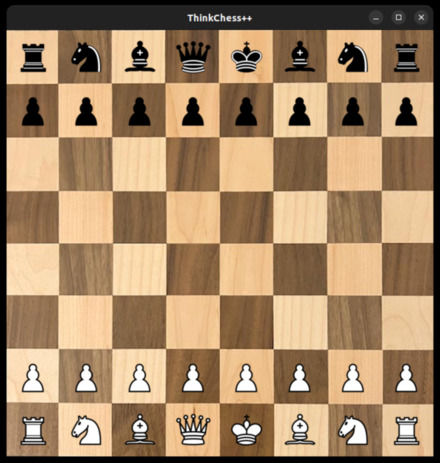
\includegraphics[width=.5\linewidth]{img/boardWithPieces.jpg}
\end{center}


\section{Showing valid moves}\label{sec:validmoves}
The goal for this section is to show the valid moves for any given piece on the board.
\subsection{Game mechanics}

For reaching our goal, we first need a way to process user input.
With SFML this is done inside the event loop of the main function:

\begin{cpp*}{linenos}
      // in event loop
      // mouse button pressed
      if (event.type == sf::Event::MouseButtonPressed) {
        if (event.mouseButton.button == sf::Mouse::Right) {
          pair<int, int> f =
            getField(event.mouseButton.x, event.mouseButton.y);
          setValidMoves(board, board[f.first][f.second]);
        }
      }
      // mouse button released
      if (event.type == sf::Event::MouseButtonReleased) {
        if (event.mouseButton.button == sf::Mouse::Right) {
          validMoves =
            vector<vector<short>>(8, vector<short>(8, 0));
        }
      }
\end{cpp*}

Here, we check if a mouse button is pressed (3).
If so, we check wether it's the right mouse button (4).
Then, we get the coordinates of the corresponding field on the board (5-6), and
fill another vector matrix with the computed valid moves for the piece under the
mouse cursor (7).

When the right mouse button is released (11-12), we reset the vector matrix of
valid moves (13-14).

In order for that to work, we need the following definitions in the main file,
just before entering the main function:

\begin{cpp*}{linenos}
vector<vector<short>> validMoves(8, vector<short>(8, 0));

void setValidMoves(vector<vector<Piece*>>& bd, Piece* pc) {
  if (!pc) return;
  for (int row = 0; row < 8; row++) {
    for (int col = 0; col < 8; col++) {
      if (pc->isValid(bd, row, col)) {
        auto current = bd[row][col];
        if (!current) validMoves[row][col] = 1; 
        else if (pc->isWhite() != current->isWhite())
          validMoves[row][col] = 2;
      }
    }
  }
}

pair<int, int> getField(int x, int y) {
  int fx = x / 80;
  int fy = y / 80;
  auto field = make_pair(fy, fx);
  return field;
}

\end{cpp*}

The work is done inside the \mintinline{cpp}{setValidMoves} function (3):\\
if there's no piece at the given coordinates, do nothing (4).
Otherwise, iterate over all fields of the board (5-6), and check wether this position can be
reached by the piece under the mouse cursor (7).
If so, get the piece of the current search position (8).
If there is no piece at this position, set this position to valid (9).
Otherwise, check the color of the current piece and if it's different from the piece
under the cursor (i.e. it can be captured), set it to valid with the special marker 2 (11).

Our \emph{object-oriented} design is starting to pay off, as we don't need to define any
game logic inside the main application file!

The last thing to do, is to draw the content of the \mintinline{cpp}{validMoves}
vector inside the main game loop (directly after drawing the pieces):

\begin{cpp*}{linenos}
  // before game loop
  sf::CircleShape valid(20.f);

    // inside game loop
    // draw valid moves
    for (int row = 0; row < 8; row++) {
      for (int col = 0; col < 8; col++) {
        if (validMoves[row][col] > 0) {
          valid.setPosition(col*80.f + 20.f, row*80.f + 20.f);
          if (validMoves[row][col] > 1)
            valid.setFillColor(sf::Color(0, 200, 0, 200));
          else valid.setFillColor(sf::Color(100, 200, 0, 100));
          window.draw(valid);
        }
      }
    }
\end{cpp*}

We iterate over all fields of the board (6-7), and if \mintinline{cpp}{validMoves} contains
an entry at this position (8), we set the marker \mintinline{cpp}{valid} on the board (9).
As an extra feature, we set the marker to a brighter color, if the piece at this postion can be
captured (10-11).
Finally, we draw the marker on the board (13).

With that, all valid moves for a selected piece are displayed while pressing the right mouse button
(with a green circular shape on the board). As soon as you release the mouse botton, the
\mintinline{cpp}{validMoves} vector is reset, and there's nothing more to draw for the next frame.

That's all for the mechanics of the game for now. Of course, we still need to implement the
\mintinline{cpp}{isValid} function for every piece, which leads us to the next section.

\subsection{Movement of the pieces}\label{subsec:validmoves}
\subsubsection{The King}

Let's start with the \emph{King}: it can move one step in any direction (on ranks, files and
diagonals), provided the target field is not occopied by a piece of the same color:

\begin{center}
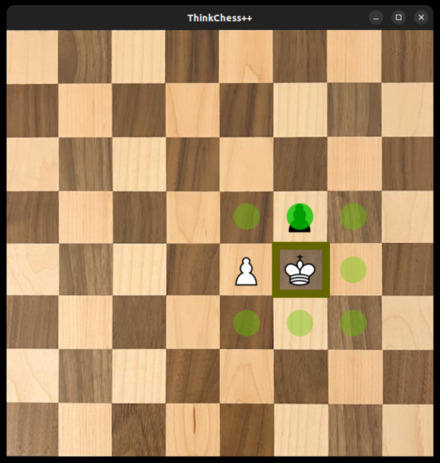
\includegraphics[width=.5\linewidth]{img/king.jpg}
\end{center}

Observe, that the piece, for which the valid moves are shown (the king on \texttt{f4}), is marked
with a dark green frame.
We will learn how to set this marker in section~\ref{sec:makemoves}, so when progamming along,
you will not see this marker for now.

If the target field is occopied by a piece of the other color (the black pawn on \texttt{f5}),
the king can capture that piece, indicated by a brighter color of the green marker.

But notice: the king is the only piece on the board that is not allowed to move to a field,
where it is immediately attacked, as it would put
itself into a \emph{check} position, and the game would be over.
We're not taking this special case into account yet, so the field \texttt{g4},
which is attacked by the black pawn, is still marked as valid.

Besides that, there's also a special move involving the king, called \emph{castling},
which we will cover in section~\ref{sec:specmoves}.

The function \mintinline{cpp}{isValid} for the king is implemented in the file
\texttt{app/pieces.cpp}:

\begin{cpp*}{linenos}
#include "pieces.hpp"
#include <vector>
using namespace std;

bool King::isValid(vector<vector<Piece*>>& bd, int r, int c) {
  bool valid = abs(r-row) <= 1 && abs(c-col) <= 1;
  return valid;
}
\end{cpp*}

First, we have to include the header file located at \texttt{include/pieces.hpp} (1),
in order to make the type definitions of the pieces available.
Observe, that we don't have to spell out the complete path to that file, thanks to these
instructions of our \texttt{CMakeLists.txt} file:

\begin{cpp}
add_executable(ThinkChess app/main.cpp app/pieces.cpp)
target_include_directories(ThinkChess PUBLIC include)
\end{cpp}

The function \mintinline{cpp}{isValid} is actually defined as
\mintinline{cpp}{King::isValid} (5), which defines the function as a member function of the
type \mintinline{cpp}{King}.
It returns \mintinline{cpp}{true} only if the given coordinates can be reached within one step.

\subsubsection{The Knight}
The \emph{Knight} is also a very special piece in one sense: it is the only piece, able to
jump over any other piece on the board.
It can move like so: either two fields on a rank and one on a file, or two on a file and one on
a rank.
That leads to an L shape for every move:

\begin{center}
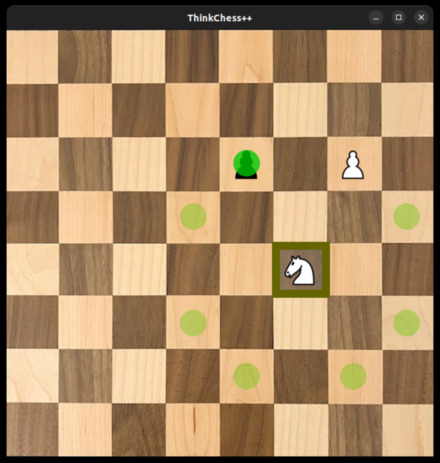
\includegraphics[width=.5\linewidth]{img/knight.jpg}
\end{center}

Observe that a knight, placed on a dark field, can reach only light fields, and vice versa.

Its \mintinline{cpp}{isValid} function is implemented like so:

\begin{cpp}
bool Knight::isValid(vector<vector<Piece*>>& bd, int r, int c) {
  bool valid = (abs(r-row) == 1 && abs(c-col) == 2) ||
               (abs(r-row) == 2 && abs(c-col) == 1);
  return valid;
}
\end{cpp}

\subsubsection{The Rook}
The \emph{Rook} moves any distance on its current rank or file, but cannot jump over any other piece.

\begin{center}
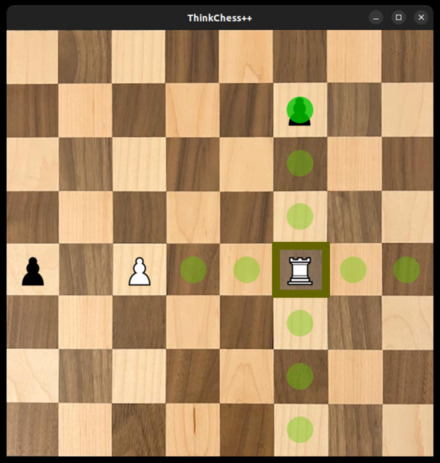
\includegraphics[width=.5\linewidth]{img/rook.jpg}
\end{center}

As the rooks movement is limited by other pieces on its way, we have to take those pieces
into account for implementing its \mintinline{cpp}{isValid} function:

\begin{cpp*}{linenos}
bool Rook::isValid(vector<vector<Piece*>>& bd, int r, int c) {
  bool valid = r == row || c == col;
  if (r == row && abs(c-col) > 1) { // same row
    if (c < col) { // left
      for (int cc = c+1; cc < col; cc++) {
        auto pc = bd[r][cc];
        if (pc) { valid = false; break; }
      }
    } else { // right
      for (int cc = col+1; cc < c; cc++) {
        auto pc = bd[r][cc];
        if (pc) { valid = false; break; }
      }
    }
  }
  if (c == col && abs(r-row) > 1) { // same column
    if (r < row) { // top
      for (int rr = r+1; rr < row; rr++) {
        auto pc = bd[rr][c];
        if (pc) { valid = false; break; }
      }
    } else { // down
      for (int rr = row+1; rr < r; rr++) {
        auto pc = bd[rr][c];
        if (pc) { valid = false; break; }
      }
    }
  }
  return valid;
}
\end{cpp*}

First, we set the result to \mintinline{cpp}{valid} if the given field it is on the same row
or column as the rook(2).\\
Then, we check for two cases:
\begin{itemize}
  \item the field is on the same row (3), or
  \item the field is on the same column (16).
\end{itemize}

In both cases, we check wether there is another piece between the field and the rook by
iterating over all those fields on that row, respective column.
If so, we set \mintinline{cpp}{valid} to \mintinline{cpp}{false} and stop the search (7, 12, 20, 25).

We have four searches, for every direction the rook can move: up, down, left, right.
But only one of them will ever be executed for any given field: either on the same row \emph{or}
on the same column.
As the search-space is very small for each search (at most 6 checks), we can consider this as a
\emph{constant time} search, or in asymptotic notation $\mathcal{O}(1)$.

\subsubsection{The Bishop}
The \emph{Bishop} can move any distance along the diagonals, on which it is placed,
unless its way is blocked by another piece:

\begin{center}
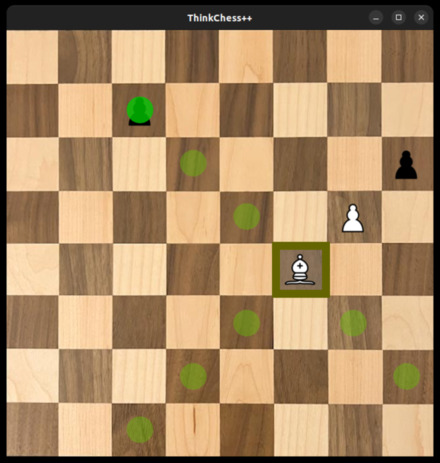
\includegraphics[width=.5\linewidth]{img/bishop.jpg}
\end{center}

Notice, that a bishop, placed initially on a light field, will always stay on a light field,
and vice versa.
Thus, both players each have a \emph{dark} and a \emph{light} bishop (the white bishop on
\texttt{f4} is a \emph{dark} bishop with its initial position on \texttt{c1}).
Dark and light bishops can never attack each other.

We use essentially the same logic as for the rook, but this time we check for pieces on
the same diagonal:

\begin{cpp}
bool Bishop::isValid(vector<vector<Piece*>>& bd, int r, int c) {
  bool valid = r-c == row-col || r+c == row+col;
  if (r-c == row-col) { // same major diagonal
    if (r < row) { // upper
      for (int rr = row-1; rr > r; rr--) {
        for (int cc = col-1; cc > c; cc--) {
          if (rr-cc == row-col) {
            auto pc = bd[rr][cc];
            if (pc) { valid = false; break; }
          }
        }
      }
    } else { // lower
      for (int rr = row+1; rr < r; rr++) {
        for (int cc = col+1; cc < c; cc++) {
          if (rr-cc == row-col) {
            auto pc = bd[rr][cc];
            if (pc) { valid = false; break; }
          }
        }
      }
    }
  }
  if (r+c == row+col) { // same minor diagonal
    if (r < row) { // upper
      for (int rr = row-1; rr > r; rr--) {
        for (int cc = col+1; cc < c; cc++) {
          if (rr+cc == row+col) {
            auto pc = bd[rr][cc];
            if (pc) { valid = false; break; }
          }
        }
      }
    } else { // lower
      for (int rr = row+1; rr < r; rr++) {
        for (int cc = col-1; cc > c; cc--) {
          if (rr+cc == row+col) {
            auto pc = bd[rr][cc];
            if (pc) { valid = false; break; }
          }
        }
      }
    }
  }
  return valid;
}
\end{cpp}

Here, we also have four searches: two for the major diagonal and another two for the minor
diagonal.
The searches are now nested loops, as we need to get both coordinates for the current field.
There are at most $6 \times 6 = 36$ tests per search, and on average only $3 \times 3 = 9$
tests for each.
And, as before, only one of these searches will ever by executed for any given field.
So, we may consider these searches as \emph{constant time} searches as well.

\subsubsection{The Queen}
The \emph{Queen} can move any distance in all directions (on its rank, file or diagonals),
only limited by other pieces in its way.
In the image below you can see, why the queen is the strongest piece on the board:

\begin{center}
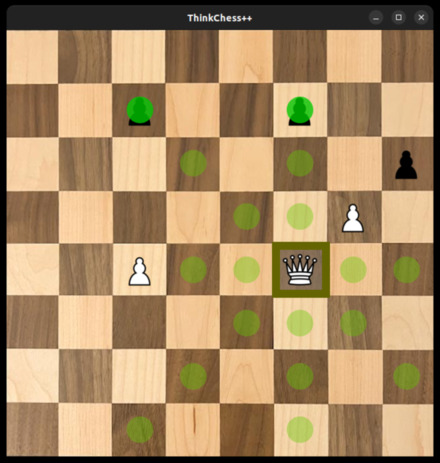
\includegraphics[width=.5\linewidth]{img/queen.jpg}
\end{center}

We use a little trick to get the queens valid moves: as the queen can move like a rook
\emph{and} a bishop, we just check for valid moves for \emph{either} of them:

\begin{cpp}
bool Queen::isValid(vector<vector<Piece*>>& bd,int r,int c) {
  auto rook = new Rook(white, row, col);
  auto bishop = new Bishop(white, row, col);
  bool valid = rook->isValid(bd, r, c) || bishop->isValid(bd, r, c);
  delete rook;
  delete bishop;
  return valid;
}
\end{cpp}

Observe that we have to delete those dummy pieces, in order to prevent any memory leaks.

\subsubsection{The Pawn}
The last piece to cover is the \emph{Pawn}: it is the weakest piece on the board, but in
exchange, both players have 8 of them.
The movement of the pawns is the most complex of all pieces:

\begin{itemize}
  \item \textbf{base case}: move straight forward one square on its file, if that square is vacant
  \item \textbf{capturing}: capture an opponents piece on eiher of the two squares diagonally
    in front of it
  \item \textbf{initial position}: if the pawn has not yet moved, it has the option of moving two
    squares straight forward, provided both squares are vacant.
\end{itemize}

Notice that the terms \emph{forward} and \emph{in front} always refer to the direction towards
the opponents pieces: the \emph{white} pawns moves to the higher ranks (e.g. \texttt{e2-e4}),
while the \emph{black} pawns move towards the lower ranks (e.g. \texttt{d3xe2}).

\begin{center}
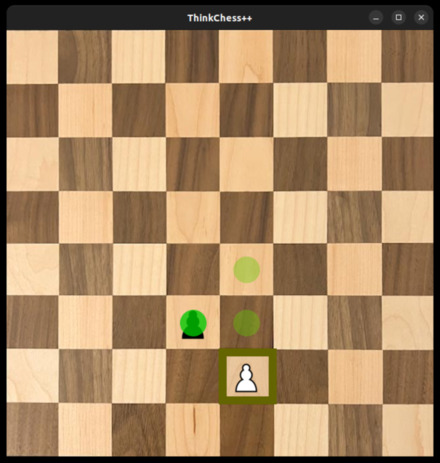
\includegraphics[width=.5\linewidth]{img/pawn.jpg}
\end{center}

There are also two special moves involving pawns, called \emph{en passant} and \emph{promotion},
which we will cover in section~\ref{sec:specmoves}.

Here's the code to put the rules in action:

\begin{cpp*}{linenos}
bool Pawn::isValid(vector<vector<Piece*>>& bd, int r, int c) {
  bool valid = false;
  if (white) {
    if (r == row-1 && c == col) { // move
      auto pc = bd[r][c];
      if (!pc) valid = true;
    }
    if (row == 6 && r == 4 && c == col) { // initial move
      auto pc = bd[r][c];
      if (!pc) valid = true;
    }
    if (r == row-1 && (c == col-1 || c == col+1)) { // capture
      auto pc = bd[r][c];
      if (pc && pc->isWhite() != white) valid = true;
    }
  } else { // black
    if (r == row+1 && c == col) { // move
      auto pc = bd[r][c];
      if (!pc) valid = true;
    }
    if (row == 1 && r == 3 && c == col) { // initial move
      auto pc = bd[r][c];
      if (!pc) valid = true;
    }
    if (r == row+1 && (c == col-1 || c == col+1)) { // capture
      auto pc = bd[r][c];
      if (pc && pc->isWhite() != white) valid = true;
    }
  }
  return valid;
}
\end{cpp*}

We have to consider white and black pawns separately, as they move in different directions (3, 16).
If there's no piece in front of the pawn, it can move to that field (6, 19).
If the pawn is on its initial position (8, 21), it also can move two squares ahead, if that field
isn't occopied (10, 23).
If there's a piece diagonal in front of the pawn (12, 25), it can be captured, if it is of the
other color (14, 27).

\chapter{Play the Game}

Now that we have a board with the pieces on it, we actually want to play the game.

To that goal, we will explore how to make moves and store them for later usage.
Finally, we will consider special moves and positions to improve the game play.

\section{Making Moves}\label{sec:makemoves}

The first thing, we need for making moves, is a way to process user input.
We'll do that inside the event loop of the main fuction:

\begin{cpp*}{linenos}
// mouse button pressed
if (event.type == sf::Event::MouseButtonPressed) {
  if (event.mouseButton.button == sf::Mouse::Left) {
    pair<int, int> f = getField(event.mouseButton.x,
                                event.mouseButton.y);
    if (touched.first == -1) touched = f;
    else if (f == touched) touched = {-1, -1};
  }
}
// mouse button released
if (event.type == sf::Event::MouseButtonReleased) {
  if (event.mouseButton.button == sf::Mouse::Left) {
    pair<int, int> f = getField(event.mouseButton.x,
                                event.mouseButton.y);
    if (touched.first != -1 && touched != f)
      makeMove(board, moves, captured, touched, f, player);
  }
}

// get board coordinates
pair<int, int> getField(int x, int y) {
  int fx = x / 80;
  int fy = y / 80;
  auto field = make_pair(fy, fx);
  return field;
}
\end{cpp*}

We're using the \emph{left} mouse button for making moves (3, 12); remember that we've
used the right button for showing valid moves.\\
First, we need the coordinates of the board, where the mouse button was pressed (4),
respectively released (13).

When \emph{pressing} the button, and no field was touched yet (6), we set the variable\\
\mintinline{cpp}{pair<int,int> touched} to those coordinates.\\
But if a field was already touched, and it's the current field, we reset
\texttt{touched} (7).

When \emph{releasing} the button, we check wether a field was touched (15), and if it's not
the current field, we make a move from the touched to the current field (16).

With this mechanism, we can make a move in two ways:
\begin{itemize}
  \item \emph{drag-and-drop}: just move a piece from its current position to the target,
    while holding the left mouse button;
  \item \emph{click twice}: click once on the piece to move, and a second time on the
    target field.
\end{itemize}

The \mintinline{cpp}{getField()} function (21-26) converts the coordinates of the mouse cursor to
the coordinates of the board matrix.
Observe that it returns the coordinates in that order: first the row index, second the
column index.

In order to clean up the design, I decided to do some refactorings: I moved all function definitions,
except the main function, to a speparate implementation file
\texttt{app/moves.cpp}; and I moved all variable definitions into the main function, to get rid of
global variables.
So, we'll have the following definitions inside the main fuction:

\begin{cpp*}{linenos}
// matrix of pieces representing the board
vector<vector<Piece*>> board(8, vector<Piece*>(8));

// matrix of valid moves for display
vector<vector<short>> validMoves(8, vector<short>(8, 0));

// list of moves, used as a stack
auto* moves = new list::List<string>;

// list of captured pieces, used as a stack
auto* captured = new list::List<Piece*>;

// touched field for making moves
pair<int, int> touched{-1, -1};

// player to turn, starting with white
bool player = true;
\end{cpp*}

The variables \texttt{moves} and \texttt{captures} are \emph{linked lists}, which I've implemented
in a separate library called \texttt{datastructures} within a namespace \texttt{list}.
I will not go into details here, but if you are interested in implementing a linked list for yourself,
have a look at the file \texttt{include/list.hpp} in that directory (it's quite well documented,
so you should find your way around).

But now, to the most important function of this section: \mintinline{cpp}{makeMove()}.

\begin{cpp*}{linenos}
void makeMove(vector<vector<Piece*>>& bd,
              list::List<string>* mv,
              list::List<Piece*>* cp,
              pair<int, int>& td,
              pair<int, int> to,
              bool& player)
{
  auto pcf = bd[td.first][td.second];
  auto pct = bd[to.first][to.second];
  bool cap = false;
  if (!pcf) {
    cout << "no piece under cursor\n";
    td = {-1, -1};
    return;
  }
  if (pcf->isWhite() != player) {
    cout << "it's not your turn\n";
    td = {-1, -1};
    return;
  }
  if (pcf->isValid(bd, to.first, to.second)) {
    if (pct && pct->isWhite() != pcf->isWhite()) {
      cap = true;
      pct->capture();
      cp->push_front(pct);
    } else if (pct) {
      cout << "illegal move!\n";
      td = {-1, -1};
      return;
    }
    mv->push_front(convertFromBoard(cap, pcf, to));
    bd[to.first][to.second] = pcf;
    bd[td.first][td.second] = nullptr;
    pcf->makeMove(to.first, to.second);
    td = {-1, -1};
    player = !player;
    cout << mv->peek(1) << "\n";
  // illegal move
  } else {
    cout << "illegal move!\n";
    td = {-1, -1};
  }
}
\end{cpp*}

First, we get the pieces of the start (\texttt{td}, the touched field) and target coordinates (\texttt{to})
of the move(8, 9).\\
If there's no piece at the start coordinates (11), reset the touched field (13) and abort the move (14).\\
If the color of the start piece doesn't match the player, whose turn it is (16), also abort the move (19).

Otherwise, check wether the move is valid (21), and wether the piece at the target position can be
captured (22).\\
If so, capture the piece (24) and and push it onto the stack of captured pieces (25).\\
Otherwise, if there's a piece of the same color (26), abort the move (29).

So far, we've checked all the possible variations and have a valid move; thus, we add the move to the
stack of moves (31).\\
Then, we set the piece under the cursor to its target position on the board (32), overwriting the old
reference, and delete its old postion (33).

Finally, we tell the piece its new position (34), reset the touched field (35), and switch to the other
player (36).

For pushing the move onto the moves stack, I used a function \mintinline{cpp}{convertFromBoard} (31),
which is defined like so:

\begin{cpp}
string convertFromBoard(bool cap, Piece* from, pair<int, int> to) {
  string move;
  char type = from->getType();
  if (type != 'P') {
    move.append(1, type);
  }
  move.append(1, colToFile(from->getCol()));
  move.append(1, rowToRank(from->getRow()));
  if (cap) {
    move.append(1, 'x');
  } else {
    move.append(1, '-');
  }
  move.append(1, colToFile(to.second));
  move.append(1, rowToRank(to.first));
  return move;
}

char colToFile(int col) {
  char file = 97 + col;
  return file;
}

char rowToRank(int row) {
  char rank = 56 - row;
  return rank;
}
\end{cpp}

The function takes a piece (\texttt{from}) and target coordinates (\texttt{to}) as parameters,
and converts them into a string of
\href{https://en.wikipedia.org/wiki/Algebraic_notation_(chess)}{algebraic chess notation}.\\
It makes use of two helper functions \mintinline{cpp}{colToFile()} and \mintinline{cpp}{rowToRank()},
which convert the coordinates of the board matrix to chess coordinates.

Those functions use a little trick, based on the specification of the \mintinline{cpp}{char} type in
C\textsuperscript{++}: the actual value of a character is stored as a \mintinline{cpp}{short int},
based on the ascii code for that character.
So, the letter `a' is stored internally as 97, and the digit `8' as 56. We use this fact for a
simple calculation.

The only thing left to do is to adjust the \mintinline{cpp}{resetBoard()} function to take care of
the moves stack and the captured pieces:

\begin{cpp}
void resetBoard(vector<vector<Piece*>>& bd,
                 list::List<string>* mv,
                 list::List<Piece*>* cp)
{
  // reset moves and captured pieces
  delete mv;
  mv = new list::List<string>;
  delete cp;
  cp = new list::List<Piece*>;
  // reset board
  for (auto rank : bd) {
    for (auto piece : rank) {
      delete piece;
    }
  }
  // --- snip ---
}
\end{cpp}

We have to explicitly delete the moves stack and the stack of captured pieces when resetting to board,
in order to avoid memory leaks.
But then, we have to create them again as empty lists, as we want to use them for the next game.
Notice, that not only the references to those lists are deleted, but also all elements inside the lists,
due to that destructor in the file \texttt{datastructures/include/list.hpp}:

\begin{cpp}
template<typename T>
class List : public LL<T> {
public:
  ~List() {
    Node* node = head;
    while(node) {
      Node* curr = node;
      node = node->next;
      delete curr;
    }
    delete node;
  }
}
\end{cpp}

The very last thing, we want to do in this section, is to add a marker inside the main function for the
touched piece on the board

\begin{cpp}
sf::RectangleShape frame(sf::Vector2f(63.f, 60.f));
frame.setFillColor(sf::Color(200, 200, 200, 50));
frame.setOutlineThickness(12.f);
frame.setOutlineColor(sf::Color(100, 100, 0));
\end{cpp}

and draw it together with the pieces inside the game loop:

\begin{cpp}
// draw pieces
for (int row = 0; row < 8; row++) {
  for (int col = 0; col < 8; col++) {
    if (board[row][col]) {
      auto piece = board[row][col];
      // --- snip ---
      if (row == touched.first && col == touched.second) {
        frame.setPosition(col*80.f + 10.f, row*80.f + 10.f);
        window.draw(frame);
      }
      pc.setPosition(col*80.f + 10.f, row*80.f + 10.f);
      window.draw(pc);
    }
  }
}
\end{cpp}

\section{Special Positions}\label{sec:specpos}
\subsection{Check and checkmate}

The most prominent position in a game is the \href{https://en.wikipedia.org/wiki/Check_(chess)}{check},
where the king is under immediate attack.
So far, we have no mechanism to respond to or even detect a \emph{check}.
Let's change that now.

For that, we only need to iterate over all opponent pieces, and if any of them can reach the king
with a valid move, we have a check:

\begin{cpp*}{linenos}
bool check(vector<vector<Piece*>>& bd, bool white) {
  Piece* king;
  bool check = false;
  for (int row = 0; row < 8; row++) {
    for (int col = 0; col < 8; col++) {
      auto current = bd[row][col];
      if (current && current->getType() == 'K' &&
          current->isWhite() == white)
      {
        king = current;
      }
    }
  }
  for (int row = 0; row < 8; row++) {
    for (int col = 0; col < 8; col++) {
      auto current = bd[row][col];
      if (current && current->isWhite() != white) {
        if (current->isValid(bd, king->getRow(), king->getCol())) {
          check = true;
        }
      }
    }
  }
  return check;
}
\end{cpp*}

First, iterate over all positions of the board (4-5) and check wether the piece at that position
is the king of the given color (7-8).
If so, store the position of the king (10).

Then, iterate again over all positions of the board (14-15) and check wether there's a piece
of the opponent color (17).
If so, check wether this piece can reach the king with a valid move (18), and if it can,
set the position to \emph{check} (19).

With that, we have two searches with 64 tests each, and we need to run them sequentially,
resulting in 128 tests.
Now you could think that's superfluous, as we could test only against the piece actually beeing
moved, reducing the second search to a single test.
But you would be wrong: a check can be given by any other piece, if a blocking piece is moved.
Convince yourself with this diagram:

\begin{center}
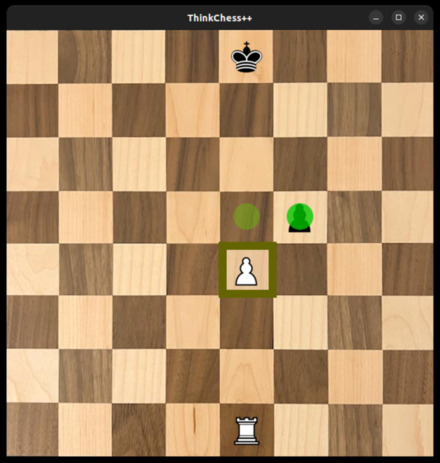
\includegraphics[width=.5\linewidth]{img/check.jpg}
\end{center}

If white captures the black pawn on \texttt{f5} with \texttt{e4xf5+}, the white rook on the
\texttt{e}-file will give the black king check.

Now, before making the move, let's look at the other special (and terminal) position: \emph{checkmate}.
If a player, given check in the last move, cannot respond to the check in the very next move, that
players king is checkmate, and the game is over.

There are, in general, three ways to get out of check:

\begin{enumerate}
  \item capturing the checking piece
  \item moving the king
  \item blocking the check.
\end{enumerate}

It's the players duty to analyze the position and to find the best solution.
For now, our app cannot do this, it's a quite complex task.\\
But thankfully, it doesn't have to: we only want to detect a checkmate and decide wether the game
is over at this point.\\
For that, we dont't need any fancy algorithm or some kind of intelligence, we just use a
\href{https://en.wikipedia.org/wiki/Brute-force_search}{brute-force} search.
Instead of finding the best solution, we only need to know if there is \emph{any} solution:

\begin{cpp*}{linenos}
bool resolveCheck(vector<vector<Piece*>>& bd, bool white) {
  for (int row = 0; row < 8; row++) {
    for (int col = 0; col < 8; col++) {
      auto current = bd[row][col];
      // get every piece of given color
      if (current && current->isWhite() == white) {
        for (int rr = 0; rr < 8; rr++) {
          for (int cc = 0; cc < 8; cc++) {
            if (current->isValid(bd, rr, cc)) {
              auto pct = bd[rr][cc];
              if (!pct || pct->isWhite() != white) {
                // make move and test for check
                bd[rr][cc] = current;
                current->makeMove(rr, cc);
                if (!check(bd, white)) {
                  bd[rr][cc] = pct;
                  current->makeMove(row, col);
                  return true;
                } else {
                  bd[rr][cc] = pct;
                  current->makeMove(row, col);
                }
              }
            }
          }
        }
      }
    }
  }
  return false;
}
\end{cpp*}

Iterate over all fields of the board (2-3); if there's a piece at this postion with the color of the
checked player (6), start another nested loop (7-8) to get the valid moves of that piece (9).\\
If the reachable fields are empty or the pieces at these positions are of the other color
(i.e. they can be captured), make this move by setting the current piece to this position (13-14).

If this new position is not giving check (15), we have a solution and return \mintinline{cpp}{true},
indicating that the check could be resolved with that move (18).\\
But, before doing so, reset the board to its original state, as we don't want to actually make
the move (16-17).

If the new position still is giving check (19), reset the board as well (20-21) and continue the search.

With that, we have four nested loops with $8 \times 8 \times 8 \times 8 = 64 \times 64 = 4096$ tests,
which is the cost of \emph{brute search}.
But, real work is only done, if we have a piece of the given color (outer nested loops), and if
this piece has any valid moves (inner nested loops).\\
A player has at most 16 pieces on the board, and assuming that each of them has 3 valid moves
on average, the \texttt{check} function will be called mo more than 48 times on average.
Thus, we may consider that search as of constant time as well.

With all that in place, we can finally make a move, while testing for \emph{check} and \emph{checkmate}:

\begin{cpp*}{linenos}
void makeMove(vector<vector<Piece*>>& bd,
              list::List<string>* mv,
              list::List<Piece*>* cp,
              pair<int, int>& td,
              pair<int, int> to,
              bool& player,
              pair<int, int>& checkmate)
{
  auto pcf = bd[td.first][td.second];
  auto pct = bd[to.first][to.second];
  bool cap = false;
  if (!pcf) {
    cout << "no piece under cursor\n";
    td = {-1, -1};
    return;
  }
  if (pcf->isWhite() != player) {
    cout << "it's not your turn\n";
    td = {-1, -1};
    return;
  }
  // valid move?
  if (pcf->isValid(bd, to.first, to.second)) {
    // can capture?
    if (pct && pct->isWhite() != pcf->isWhite()) {
      cap = true;
      cp->push_front(pct);
    } else if (pct) { // same color
      cout << "illegal move!\n";
      td = {-1, -1};
      return;
    }
    // legal move
    string move = convertFromBoard(cap, pcf, to);
    bd[to.first][to.second] = pcf;
    bd[td.first][td.second] = nullptr;
    pcf->makeMove(to.first, to.second);
    // check?
    if (check(bd, player)) { // gives itself check
      cout << "illegal move!\n";
      bd[to.first][to.second] = pct;
      bd[td.first][td.second] = pcf;
      pcf->makeMove(td.first, td.second);
      td = {-1, -1};
      return;
    }
    if (check(bd, !player)) { // gives opponent check
      if (resolveCheck(bd, !player)) {
        move.append(1, '+');
      } else { // cannot get out of check
        move.append(1, '#');
        mv->push_front(move);
        cout << mv->peek(1) << "\n";
        checkmate = getKing(bd, !player);
        return;
      }
    }
    mv->push_front(move);
    cout << mv->peek(1) << "\n";
    td = {-1, -1};
    player = !player;
  // illegal move
  } else {
    cout << "illegal move!\n";
    td = {-1, -1};
  }
}
\end{cpp*}

We have an extra parameter \mintinline{cpp}{pair<int, int>& checkmate} for keeping track of \emph{checkmate}.
Besides, There's nothing new in lines (1-37).

Then test, wether the move gives the own king check (39), and if it does, abort the move (44-45), as
this is not allowed.
But, before that, reset the already made move (41-43).
Notice, that we had to make the move in the first place in order to allow the test for check.

If the move gives the opponents king check (47), test wether the check could possibly be
resolved (48), and if so, add the marker `+' to the move (indicating check, 49).\\
If the check cannot be resolved (50), add the marker `\#' to the move (indicating checkmate, 51),
push the move to the moves stack (52), and set the \texttt{checkmate} variable to the postion
of the checkmated king (54).
Then, proceed as before (58-67).

The only thing missing, is the implementation of the \texttt{getKing} function on line 54.
It's essentially the same as the first loop of the \texttt{check} function, but only returning
the coordinates of the king.
Try to implement that function for yourself; if you get stucked, check my implementation in the
file \texttt{app/moves.cpp}.

We use the \texttt{checkmate} variable to to stop the game and draw a corresponding marker on the board
within the main function of the app:

\begin{cpp}
short state = 1;
pair<int, int> checkmate{-1, -1};

//marker for checkmate
sf::RectangleShape cm(sf::Vector2f(63.f, 60.f));
cm.setFillColor(sf::Color(200, 200, 200, 50));
cm.setOutlineThickness(12.f);
cm.setOutlineColor(sf::Color(200, 0, 0));

// game loop
while (window.isOpen()) {
  // event loop
  for (auto event = sf::Event{}; window.pollEvent(event);) {
    if (event.type == sf::Event::Closed) {
      window.close();
    }
    // game is running in play mode
    if (state == 1) {
      // mouse button pressed
      if (event.type == sf::Event::MouseButtonPressed) {
        if (event.mouseButton.button == sf::Mouse::Right) {
          pair<int, int> f =
            getField(event.mouseButton.x, event.mouseButton.y);
          setValidMoves(board, validMoves, board[f.first][f.second]);
        }
        if (event.mouseButton.button == sf::Mouse::Left) {
          pair<int, int> f =
            getField(event.mouseButton.x, event.mouseButton.y);
          if (touched.first == -1) touched = f;
          else if (f == touched) touched = {-1, -1};
        }
      }
      // mouse button released
      if (event.type == sf::Event::MouseButtonReleased) {
        if (event.mouseButton.button == sf::Mouse::Right) {
          validMoves = vector<vector<short>>(8, vector<short>(8, 0));
        }
        if (event.mouseButton.button == sf::Mouse::Left) {
          pair<int, int> f =
            getField(event.mouseButton.x, event.mouseButton.y);
          if (touched.first != -1 && touched != f)
            makeMove(board, moves, captured, touched,
                     f, player, checkmate);
        }
      }
    } // end play mode
  } // end event loop

  // draw pieces
  for (int row = 0; row < 8; row++) {
    for (int col = 0; col < 8; col++) {
      if (board[row][col]) {
        // --- snip ---
        if (row == checkmate.first && col == checkmate.second) {
          cm.setPosition(col*80.f + 10.f, row*80.f + 10.f);
          window.draw(cm);
        }
        pc.setPosition(col*80.f + 10.f, row*80.f + 10.f);
        window.draw(pc);
      }
    }
  }
  // display frame
  window.display();

  // stop game when checkmate
  if (checkmate.first != -1) state = 0;
\end{cpp}

And here you have it: a fully playable chess app for two players!

Playing the moves
\begin{verbatim}
1. e2-e4 e7-e5
2. Ng1-f3 Ng8-f6
3. Nf3xe5 Nf6xe4
4. Qd1-f3 Ne4-c5
5. Qf3xf7#
\end{verbatim}

will lead to this position, correctly identified as checkmate (a.k.a
the \emph{Scholar's mate}):

\begin{center}
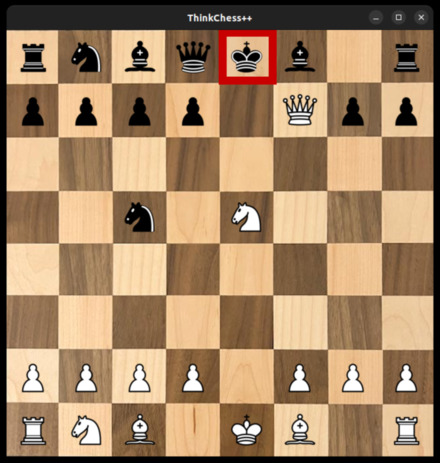
\includegraphics[width=.5\linewidth]{img/checkmate.jpg}
\end{center}

\subsection{Stalemate}\label{subsec:stale}

\href{https://en.wikipedia.org/wiki/Stalemate}{Stalemate} is a situation in chess where the player,
whose turn it is to move, is not in check but has no legal move.
Stalemate immediately results in a draw (i.e. the game is over and both players are credited half
a point).
During the endgame, stalemate is a resource that can enable the player with the inferior position
to draw the game rather than lose.

Stalemate is mucher harder to detect than checkmate: as the king has not been given check,
we cannot use our \texttt{check} and \texttt{resolveCheck} functions for this position.
Of course, we could try to do something similar, but only with a much higher expense.
But, as stalemates are actually much rarer than checkmates, I decided to not spend this effort for now.

So, when playing a game with the app, both players have to agree to stalemate (and with that to a draw),
like they would have to in a tournament.

\section{Special Moves}\label{sec:specmoves}

To complete this chapter, we will now implement the missing \emph{special} moves for
\begin{itemize}
  \item the king: \href{https://en.wikipedia.org/wiki/Castling}{castling}
  \item the pawns: \href{https://en.wikipedia.org/wiki/En_passant}{en passant} and
    \href{https://en.wikipedia.org/wiki/Promotion_(chess)}{promotion}.
\end{itemize}

\subsection{Castling}

Castling is the only move, in which two pieces are moved at once (the king and one
of the rooks of the same color).
The king moves two squares towards a rook on the same rank and the rook moves to the square
that the king passed over.

Castling is permitted only if
\begin{itemize}
  \item neither the king nor the rook has previously moved
  \item the squares between the king and the rook are vacant
  \item the king does not leave, cross over, or finish on a square attacked by an enemy piece.
\end{itemize}

\begin{center}
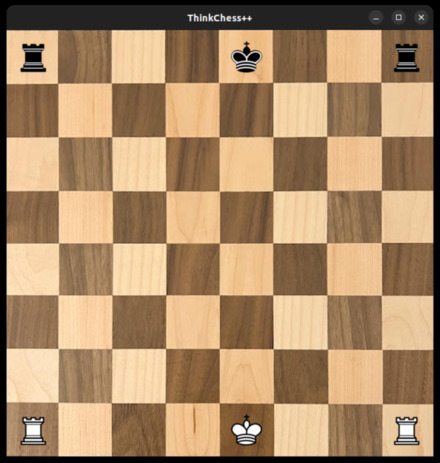
\includegraphics[width=.5\linewidth]{img/castling1.jpg}
\end{center}

Assuming in the diagramm above, that neither of the players has casteld yet, they could move
like so:

\begin{center}
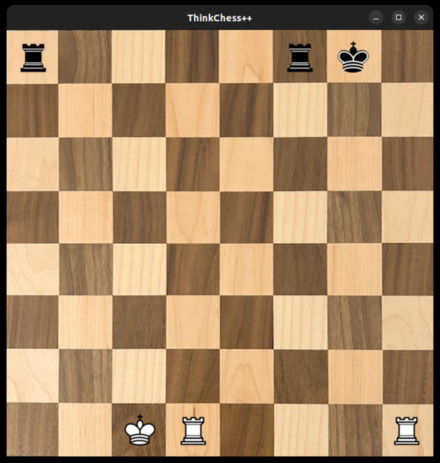
\includegraphics[width=.5\linewidth]{img/castling2.jpg}
\end{center}

White has castled to the queenside (indicated with \texttt{0-0-0}), while black has castled to
the kingside (indicated with \texttt{0-0}).

We implement the logic for \emph{castling} with a function called \texttt{castling}:

\begin{cpp*}{linenos}
char castling(vector<vector<Piece*>>& bd,
              Piece* king, pair<int, int> to)
{
  if (check(bd, king->isWhite())) return 'N'; // king is in check
  if (king->isWhite()) { // white
    if (king->getRow() == 7 && king->getCol() == 4) {
      // TODO: king has not yet moved
      if (to.first == 7 && to.second == 6) { // kingside
        auto rook = bd[7][7];
        if (!rook || rook->getType() != 'R'
                  || rook->isWhite() != king->isWhite()) {
          // TODO: rook has moved
          return 'N';
        }
        auto pc1 = bd[7][5];
        auto pc2 = bd[7][6];
        if (pc1 || pc2) return 'N'; // fields occupied
        else {
          // test for check
          bd[7][5] = king;
          king->makeMove(7, 5);
          if (check(bd, king->isWhite())) {
            bd[7][4] = king;
            king->makeMove(7, 4);
            bd[7][5] = nullptr;
            return 'N';
          } else {
            bd[7][4] = king;
            king->makeMove(7, 4);
            bd[7][5] = nullptr;
          }
          bd[7][6] = king;
          king->makeMove(7, 6);
          if (check(bd, king->isWhite())) {
            bd[7][4] = king;
            king->makeMove(7, 4);
            bd[7][6] = nullptr;
            return 'N';
          } else {
            bd[7][4] = king;
            king->makeMove(7, 4);
            bd[7][6] = nullptr;
          }
          return 'K';
        }
      } else if (to.first == 7 && to.second == 2) {
      // --- snip queenside ---
      }
    }
  } else {
  // --- snip black ---
  }
  return 'N';
}
\end{cpp*}

First, test wether the king is currently in check, and if so, abort with negative result (4).
Then, test for the white king (5): we have to test the kings separately, as they sit on different ranks.

Next, test wether the king is on its initial position (6).
Observe, that for now, this test is not complete: the king could have moved from and back to its initial
position.
Since we will learn to process stored moves only in the next chapter, there is no way to complete the
test for now.
But we must not forget to make this right, so I've left a \texttt{TODO} comment here.

Next, test for kingside castling (8): if there's no rook of the same color on its initial position (10-11),
abort with negative result (13).
Observe, that we have the same issue as with the king before, so I've added a \texttt{TODO} marker as well.

Then, test wether the fields between the king and the rook are occopied (17), and if not, continue
with the tests for check for these fields (18).
For that, we move the king to the first field (20-21) and test for check (22).
If it is in check, abort with negative result (26), after undoing the king move (23-25), since we don't
want to actually move the king.
Otherwise reset the move as well (27-31), and test the second field for check (32-43), following the logic
from the first field.

If there are no pieces at both fields, and the king would not be in check at those fields, return
positive result \texttt{K} for kingside castling (44).

Then, repeat the process for queenside castling (46), and finally both processes for the black king (51).
If no valid castling position was found, return negative result (53).

With that, we have a lot of redundant code, only differing in the ranks of the king.
Of course, one could write that in a more compact way.
But that could lead to an overly clever solution, which would be hard to understand for someone without
implicit knowledge of what's going on, even for your future self.
So, I decided to leave the code this way and to make every step explicit.

The compiler won't care about lengthy code anyway.
On the contrary, when optimization is enabled (e.g. with the flag \texttt{-O3}),
the compiler will create the most efficient machine code possible.

By the way, if you want to compile the project in release mode with optimization enabled,
you can call \texttt{<cmake .. -DCMAKE\_BUILD\_TYPE=Release>}
from the \texttt{build} directory, followed by \texttt{<cmake -build .>}.\\
This will recompile the whole project, and every time, you call \texttt{cmake} after that, the project will be
compiled in release mode, unless you decide to delete the build directory and re-create it with
\texttt{cmake -B build} from the root folder.

Having \texttt{castling} in place, we can use it inside our \texttt{makeMove} function:

\begin{cpp*}{linenos}
// already castled, 0 = no, 1 = white, 2 = black, 3 = both
short castled = 0;

void makeMove(vector<vector<Piece*>>& bd,
              list::List<string>* mv,
              list::List<Piece*>* cp,
              pair<int, int>& td,
              pair<int, int> to,
              bool& player,
              pair<int, int>& checkmate,
              short& castled)
{
  auto pcf = bd[td.first][td.second];
  auto pct = bd[to.first][to.second];
  bool cap = false;
  if (!pcf) {
    cout << "no piece under cursor\n";
    td = {-1, -1};
    return;
  }
  if (pcf->isWhite() != player) {
    cout << "it's not your turn\n";
    td = {-1, -1};
    return;
  }
  // castling
  short cast = player ? 1 : 2;
  if (castled < 3 && castled != cast && pcf->getType() == 'K' && !pct) {
    string move = "";
    char form = castling(bd, pcf, to);
    if (form == 'K') {
      castled = castled > 0 ? 3 : cast;
      move = "0-0";
      // make king move
      bd[td.first][td.second+2] = pcf;
      pcf->makeMove(td.first, td.second+2);
      bd[td.first][td.second] = nullptr;
      // make rook move
      auto rook = bd[td.first][7];
      bd[td.first][td.second+1] = rook;
      rook->makeMove(td.first, td.second+1);
      bd[td.first][7] = nullptr;
      if (check(bd, !player)) { // gives opponent check
        if (resolveCheck(bd, !player)) {
          move.append(1, '+');
        } else { // cannot get out of check
          move.append(1, '#');
          mv->push_front(move);
          cout << mv->peek(1) << "\n";
          checkmate = getKing(bd, !player);
          return;
        }
      }
      // complete move
      mv->push_front(move);
      cout << mv->peek(1) << "\n";
      td = {-1, -1};
      player = !player;
      return;
    } else if (form == 'Q') {
      castled = castled > 0 ? 3 : cast;
      move = "0-0-0";
      // make king move
      bd[td.first][td.second-2] = pcf;
      pcf->makeMove(td.first, td.second-2);
      bd[td.first][td.second] = nullptr;
      // make rook move
      auto rook = bd[td.first][0];
      bd[td.first][td.second-1] = rook;
      rook->makeMove(td.first, td.second-1);
      bd[td.first][0] = nullptr;
      if (check(bd, !player)) { // gives opponent check
        if (resolveCheck(bd, !player)) {
          move.append(1, '+');
        } else { // cannot get out of check
          move.append(1, '#');
          mv->push_front(move);
          cout << mv->peek(1) << "\n";
          checkmate = getKing(bd, !player);
          return;
        }
      }
      // complete move
      mv->push_front(move);
      cout << mv->peek(1) << "\n";
      td = {-1, -1};
      player = !player;
      return;
    } // else do nothing and continue with check for valid move
  }
  // --- snip processing other moves ---
}
\end{cpp*}

We have a new variable \texttt{castled} inside the main function (2), and a respective parameter
in the \texttt{makeMove} function (11) for keeping track of castling.

The new part starts on line (27): we define a local variable \texttt{cast} and set it to the player,
whose turn it is.
Then we test, wether that player has already castled, and wether the piece to move is a king and the
target field is not occupied (28).
Then, test wether castling is possible for that king (30), and if it's a kingside castling (31),
do the following:
\begin{enumerate}
  \item indicate, that the player has castled (32)
  \item set the correct notation for the move (33)
  \item make the king move by setting it 2 fields to the right (35-37)
  \item make the rook move by setting it to the left of the king (39-42)
  \item test wether the move gives the opponents king check (43)
  \item if so, test wether the check could be resolved by the opponent (44)
  \item if so, complement the move's notation with a \texttt{+}
  \item otherwise, it is checkmate: complete the move and stop the game (46-52)
  \item complete the move (55-59)
\end{enumerate}

Then, repeat the steps above for queenside castling (60-89). I've left out the subsequent code, as
it does not differ from the previous version.

With that, we can perform (almost) correct castling for both players; we'll revisit the code for
the \texttt{castling} method in the next chapter.

\subsection{Promotion}

\href{https://en.wikipedia.org/wiki/Promotion_(chess)}{Promotion} is the replacement of a pawn with a
new piece when the pawn is moved to its last rank.
The player replaces the pawn immediately with a queen, rook, bishop, or knight of the same color.
The new piece does not have to be a previously captured piece.

Promotion is almost always to a queen (a.k.a \emph{queening}), as it is the most powerful piece.
Since we don't have a sufficient GUI yet (so the player cannot choose a different piece), we will
restrict promotion to queening for now.

With that restriction, it is quite easy to implement promotion inside our \texttt{makeMove} function:

\begin{cpp*}{linenos}
// valid move?
if (pcf->isValid(bd, to.first, to.second)) {
// can capture?
if (pct && pct->isWhite() != pcf->isWhite()) {
  cap = true;
  cp->push_front(pct);
} else if (pct) { // same color
  cout << "illegal move!\n";
  td = {-1, -1};
  return;
}

string move = convertFromBoard(cap, pcf, to);

// promotion
if (pcf && pcf->getType() == 'P') {
  if (pcf->isWhite() && pcf->getRow() == 1) { // white
    pcf = new Queen(1, pcf->getRow(), pcf->getCol());
    move.append("=Q");
  } else if (!pcf->isWhite() && pcf->getRow() == 6) { // black
    pcf = new Queen(0, pcf->getRow(), pcf->getCol());
    move.append("=Q");
  }
} // end promotion

// legal move
bd[to.first][to.second] = pcf;
bd[td.first][td.second] = nullptr;
pcf->makeMove(to.first, to.second);
\end{cpp*}

We have to put the new code (15-24) inside the check for valid moves, just before making the move (27-29).
The code tests wether the piece to move is a pawn (16), and wether it is currently placed on the last but one
rank for its color (17, 20).
If so, the pawn is simply replaced with a queen of the same color (18, 21) and the moves notation is
completed accordingly (19, 22).

\begin{center}
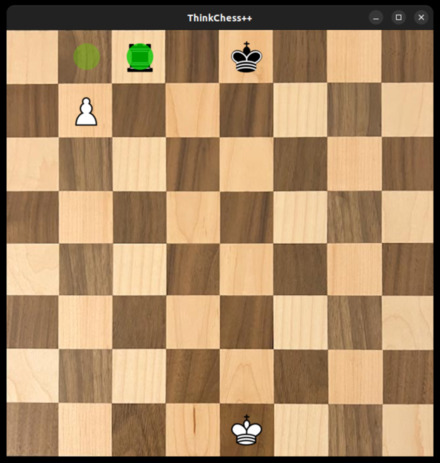
\includegraphics[width=.5\linewidth]{img/queening.jpg}
\end{center}

When the pawn on \texttt{b7} captures the rook on \texttt{c8} in the diagram above,
our app will promote the pawn to a queen and also detects the check, reporting this move:
\texttt{b7xc8=Q+}.

\subsection{En passant}

The last special move, we want to cover, is a pawns move called
\href{https://en.wikipedia.org/wiki/En_passant}{en passant}.

The move describes the capture by a pawn of an enemy pawn on the same rank and an adjacent file,
that has just made an initial two-square advance.\\
The capturing pawn moves to the square that the enemy pawn passed over, as if the enemy pawn had
advanced only one square.

The rule ensures that a pawn cannot use its two-square move to safely skip past an enemy pawn. 

But, since capturing \emph{en passant} is permitted only on the turn immediately after the
two-square advance, we would need to investigate the moves history for this.
As we have no means to do that for now, we'll implement that move only in a later chapter,
marking it with \texttt{TODO} in the meanwhile.

\section{Showing valid moves (revisited)}

In section~\ref{sec:validmoves} we learned how to show the valid moves for any piece,
by pressing the right mouse button on it.

So far, this will only display the valid moves in general, ignoring special positions
(§~\ref{sec:specpos}) and special moves (§~\ref{sec:specmoves}).
So, we will not see the moves for castling when clicking on a king, but we'll see moves,
which are not allowed in the current position (whenever the move would give check to the own king).

We could certainly resolve this, but this would also mean a major redesign of our display logic,
and would not bear any other benefits for the current game behavior.
So I decided, to leave it as it is for now.

On the bright side, this behavior has a positve didactic effect for learners: if you want to make
a move, shown as valid, and the app refuses that move (for good reasons), you have to analyze the position
for yourself and find the reason why.
In most of theses cases, you'd have missed a given check.


\chapter{Enhancing the GUI}

In this chapter we'll add a dashboard to our app, including
\begin{itemize}
  \item a \emph{timer} for keeping track of the player's thinking time
  \item an indicator for \emph{material evaluation}
  \item the display of \emph{captured pieces} for each player
  \item a \emph{move indicator} for the last move
  \item a display for the complete \emph{moves history}, and
  \item an \emph{info field} for displaying messages from the app.
\end{itemize}

We will also store the current game to a textfile for later use, and add a splash-screen,
allowing to display the result of a game and to switch the game mode.

Furthermore, we will give a player the option to take back a move, to offer a draw,
and to resign.

Finally, we'll revisit some \emph{special moves}.

With all that in place, our app will look like so:

\begin{center}
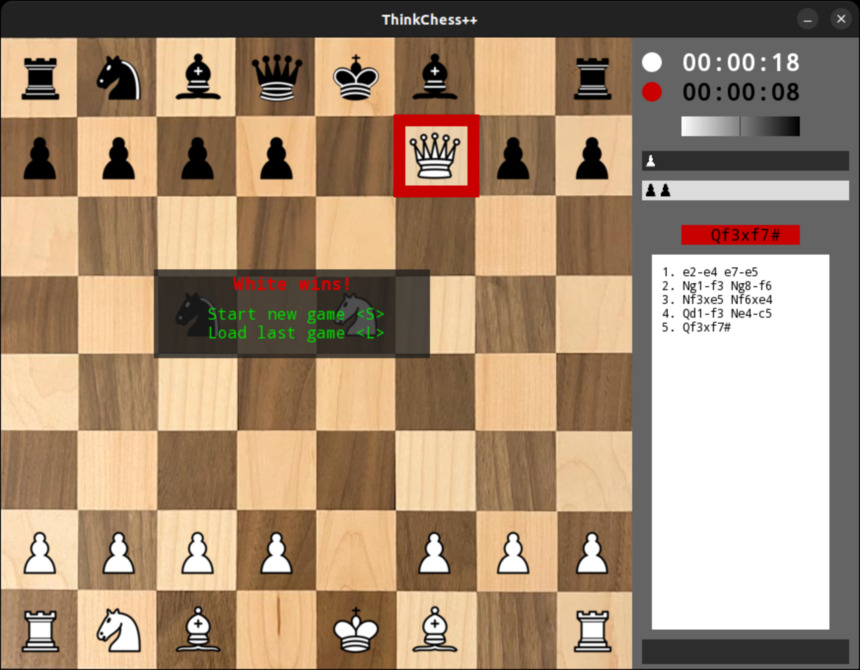
\includegraphics[width=\linewidth]{img/display.jpg}
\end{center}

\section{Refactoring}

First of all, I created a new translation unit at \texttt{app/display.cpp} and its
header file at \texttt{include/display.hpp}, which will contain all the display-oriented logic.

Next, I created another new unit at \texttt{app/position.cpp} and its header file at\\
\texttt{include/position.hpp} which contains all the move-oriented logic.\\
I moved all the functions from the old file \texttt{app/moves.cpp} to this new file and
deleted the old file.

This new file contains a new type \texttt{Position}, which holds all the position-relevant variables,
so I could delete those from the \texttt{main()} function.

\begin{cpp}
class Position {
public:
  ~Position() {}
  Position(short gs) : gamestate{gs}, player{true},
               board{8, vector<Piece*>(8)},
               mvCount{0}, castled{0}, checkmate{-1, -1},
               checked{false}, eval{0.f}
  {}

  // returns a material evaluation for both players
  void evaluate();

  // take back last move
  bool takeBackMove();

  // make a move
  bool makeMove(pair<int, int> from, pair<int, int> to);

  // gamestate: 0 = game over, 1 = 2-player, 2 = analyze 
  short gamestate;

  // player on turn, starting with white
  bool player;
  
  // matrix of pieces representing the board
  vector<vector<Piece*>> board;

  // vector of moves, used as a stack
  vector<string> moves;

  // list of captured pieces, used as a stack
  vector<Piece*> captured;

  // total count of moves
  int mvCount;
  
  // castled: 0 = no, 1 = white, 2 = black, 3 = both
  short castled;
  
  // coordinates of the piece, which gave checkmate
  std::pair<int, int> checkmate;
  
  // last move gave check
  bool checked;

  // basic evaluation of positions
  float eval;

  // infotext
  string info;
};
\end{cpp}

Observe, that I've made all the member types public, in order to avoid creating all the associated
\emph{getter} and \emph{setter} functions.
This would not be a good design decision, if we were to create a library, which was intended to
be used by different clients, as those clients could harm the game logic.
But, in our case, the only client is the \texttt{main()} function of our app, and I suppose that
we know what we are doing.

With the new type \texttt{Position} in place, we can initialize all relevant variables with a single
call from inside the main function: \mintinline{cpp}{Position position(0);} and call the
\texttt{makeMove} function with just two parameters (which are the field coordinates from the board)
like so: \mintinline{cpp}{position.makeMove(touched, to)}.

Finally, I extended the viewport of the app and made it not resizable:

\begin{cpp}
auto window = sf::RenderWindow{ {870, 640u},
                                "ThinkChess++",
                                sf::Style::Close,
                                settings };

window.clear(sf::Color(100, 100, 100));
\end{cpp}

The last line just sets the background of the display area to gray (inside the game loop).

\section{Timer}

For displaying the \emph{timer}, we first have to include the \texttt{chrono} library
and define two time counters, as well as two time points:

\begin{cpp}
#include <chrono>
using namespace chrono;

unsigned wTime = 0;
unsigned bTime = 0;
steady_clock::time_point last;
last = steady_clock::now();
steady_clock::time_point now;
\end{cpp}

For calculating the current thinking time for both player, we have this code inside the
game loop, just before drawing anything:

\begin{cpp*}{linenos}
if (position.gamestate == 1) {
  now = steady_clock::now();
  if (now - last > 1s) {
    last = steady_clock::now();
    if (position.player) wTime++;
    else bTime++;
  }
}
\end{cpp*}

The code checks, wether we are in playing mode (gamestate is set to 1), and captures the current
time point (2).
If the difference between \texttt{now} and \texttt{last} is greater than one second (3), increase
the time counter for the player whose turn it is (5-6).
Remember, we have set the \texttt{sf::FramerateLimit} to 10, so this code will be called 10 times
pers second, and we cannot simply increase the time counters for each pass.

In oder to actually draw the timer, we have this code inside the game loop (directly after the
last code snippet):

\begin{cpp*}{linenos}
string timer = "";
if (position.player) {
  window.draw(wActive);
  timer = getTime(wTime);
  wTimer.setString(timer);
} else {
  window.draw(bActive);
  timer = getTime(bTime);
  bTimer.setString(timer);
}
if (position.checkmate.first != -1) {
  if (position.player) {
    bActive.setFillColor(sf::Color(200, 0, 0));
    window.draw(bActive);
  } else {
    wActive.setFillColor(sf::Color(200, 0, 0));
    window.draw(wActive);
  }
}
window.draw(wTimer);
window.draw(bTimer);
\end{cpp*}

This code also draws the indicator for the active player (the white or black circle in front of
the timer) in lines 3 and 7.
If the app has detected a checkmate (11), the active player's indicator is set to a red color
(13, 16).

For that to work, we need to have the respective \texttt{sf::Sprite}s to be defined (before
entering the game loop):

\begin{cpp*}{linenos}
// set timer
sf::Text wTimer;
wTimer.setFont(noto);
wTimer.setCharacterSize(24);
wTimer.setStyle(sf::Text::Bold);
wTimer.setFillColor(sf::Color::White);
wTimer.setString("00:00:00");
wTimer.setPosition(690.f, 10.f);

sf::Text bTimer = wTimer;
bTimer.setFillColor(sf::Color::Black);
bTimer.setPosition(690.f, 40.f);

// marker for aktive player
sf::CircleShape wActive(10.f);
wActive.setPosition(650.f, 15.f);
wActive.setFillColor(sf::Color::White);

sf::CircleShape bActive(10.f);
bActive.setPosition(650.f, 45.f);
bActive.setFillColor(sf::Color::Black);
\end{cpp*}

In order to display text with SFML, we have to set a font to the \texttt{sf::Text} sprite (3),
and we also must have a font already in place (just before the last snippet):

\begin{cpp}
sf::Font noto;
if (!noto.loadFromFile("../img/NotoMono-Regular.ttf")) {
  cout << "failed to load the font\n";
  return 1;
}
\end{cpp}

I have chosen the \emph{NotoMono-Regular} font, because it is a fixed-space font and quite compact:
it only contains 897 glyphs (the images for actually drawing each character), in contrast to
more than 5,000 glyphs for fancier fonts.

The last thing missing is the function \texttt{getTime()} to convert a time counter (an unsigned
integer value) into a readable time format. This function is located inside the new
\texttt{app/display.cpp} implementation file:

\begin{cpp*}{linenos}
string getTime(unsigned t) {
  string result = "";
  unsigned h = 0;
  unsigned m = t / 60;
  unsigned s = t % 60;
  if (m >= 60) {
    h = m / 60;
    m = m % 60;
  }
  if (h < 10) {
    result.append(1, '0');
    result.append(to_string(h));
  } else {
    result.append(to_string(h));
  }
  result.append(1, ':');
  if (m < 10) {
    result.append(1, '0');
    result.append(to_string(m));
  } else {
    result.append(to_string(m));
  }
  result.append(1, ':');
  if (s < 10) {
    result.append(1, '0');
    result.append(to_string(s));
  } else {
    result.append(to_string(s));
  }
  return result;
}
\end{cpp*}

The logic is straight forward: just divide the total amount of seconds by 60 to get the minutes (4),
and take the ramainder of that calculation to get the remaining seconds (5).
If the resulting minutes are greater than 60 (6), repeat those steps to get the hours and remaining
minutes (7-8).
The rest of the code (10-29) is just for formatting: if hours, minutes, and seconds are less than 10,
insert the digit \texttt{0}  at the appropriate position.

\section{Material evaluation}

\emph{Material evaluation} is the first step in evaluating the players positions on the board.

Evaluating positions is a copmlex task, for which one must have a deeper understanding of
several factors, including the pawn structure, control of the center, space and initiative.
We'll explore the basics of position evaluation in the next chapter, which will also be the first
chapter mainly about \emph{playing} chess.

For now, we are only interested in the first part of this process, which is straight forward:
add up the values of the pieces of each player and compare them.

For that we need a new function, which needs access to the board; so it's
a natural choice to define it as a member of the type \texttt{Position}:

\begin{cpp}
void evaluate() {
  pair<int, int> matEval = evaluateBoard(board);
  eval = float(matEval.first) / 100
       - float(matEval.second) / 100;
}
\end{cpp}

The function calls a helper function, which is defined in the corresponding implementation file:

\begin{cpp}
pair<int, int> evaluateBoard(const vector<vector<Piece*>>& bd) {
  int white = 0;
  int black = 0;
  
  for (int row = 0; row < 8; row++) {
    for (int col = 0; col < 8; col++) {
      auto pc = bd[row][col];
      if (pc) {
        pc->isWhite() ? white += pc->getValue()
                      : black += pc->getValue();
      }
    }
  }
  pair<int, int> eval = make_pair(white, black);
  return eval;
}
\end{cpp}

Observe my design choice: I defined all functions, which need a reference to the board, but
will not modify it, as helper functions outside the class \texttt{Position}, and I made the
reference to the board \mintinline{cpp}{const}. So the compiler will ensure that indeed
no updates to the board will happen inside those functions.

I also decided to sligthly modify the value scheme for pieces of section~\ref{subsec:pieces}:
the queen now has a value of 9, and the rooks each a value of 5.
To be able to do more accurate calculations later, the values are defined as \emph{centipawns}
by multiplying them with 100.
With that, we'll be able to make all future calculations on the base of integer values,
which should be faster than calculating with \mintinline{cpp}{float} representations of the
value.

The current implementations of the pieces look like so:

\begin{cpp}
class Queen : public Piece {
public:
  ~Queen() {}
  Queen(bool w, int r, int c) :
    type{'Q'}, white{w}, value{900}, row{r}, col{c} {}

  char getType() override { return type; }
  int getValue() override { return value; }
  bool isWhite() override { return white; }
  int getRow() override { return row; }
  int getCol() override { return col; }
  void makeMove(int r, int c) override { row = r; col = c; }
  bool isValid(const vector<vector<Piece*>>& bd, int r, int c) override;

private:
  char type;
  bool white;
  int value;
  int row;
  int col;
};
\end{cpp}

Now we can use the evaluation function inside the game loop to actually draw the
\emph{evaluation meter}:

\begin{cpp*}{linenos}
if (moved) {
  if (position.mvCount % 2 == 0) {
    position.evaluate();
    eval = position.eval;
    if (eval > 10.0) {
      eval = 10.f;
      mb[2].color = sf::Color(200, 0, 0, 200);
      mb[4].color = sf::Color(200, 0, 0, 200);
      mb[5].color = sf::Color(200, 0, 0, 200);
    }
    if (eval < -10.0) {
      eval = -10.f;
      mb[0].color = sf::Color(200, 0, 0, 200);
      mb[1].color = sf::Color(200, 0, 0, 200);
      mb[3].color = sf::Color(200, 0, 0, 200);
    }
    mi[2].position = sf::Vector2f(750.f + eval*6.f, 80.f);
    mi[3].position = sf::Vector2f(750.f + eval*6.f, 100.f);
    if (eval > 0) {
      mi[2].color = sf::Color::White;
      mi[3].color = sf::Color::White;
    } else {
      mi[2].color = sf::Color::Black;
      mi[3].color = sf::Color::Black;
    }
  }
}
\end{cpp*}

When a move is complete, i.e. both players have moved (2), evaluate the material (3).
Then, set the local variable \texttt{eval} to the calculated value (4);
we are doing so, because we don't want to tinker with the member variables of
\texttt{Position} from outside the class (remember my caveat for this design decision).\\
For display purposes, we restict that value to the range $[-10, 10]$, and set the
background color of the evaluation meter to red, if the value is outside
that range (5-16).\\
Finally, we set the position and the color of the evaluation indicator (17-24).
We'll see soon, how this works.

You may have noticed that this code will only be executed, if a move was made (1).
Remember, this code is placed inside the game loop, and we don't want to evaluate the board
for every update of the display.
So I modified the \mintinline{cpp}{Position::makeMove()} function to report success, and call
it like so: \mintinline{cpp}{moved = position.makeMove(touched, to)}:

\begin{cpp}
bool makeMove(pair<int, int> td, pair<int, int> to) {
  auto pcf = board[td.first][td.second];
  auto pct = board[to.first][to.second];

  if (!pcf) {
    info = "no piece selected";
    return false;
  }
  if (pcf->isWhite() != player) {
    info = "it's not your turn";
    return false;
  }
  // --- snip ---
}
\end{cpp}

The background of the evaluation meter (\texttt{mb}) is defined as an SFML primitive
(a set of two unconnected triangles), and the evaluation indicator (\texttt{mi})
as a set of two unconnected vertical lines:

\begin{cpp*}{linenos}
sf::VertexArray mb(sf::Triangles, 6);
mb[0].position = sf::Vector2f(690.f, 80.f);
mb[1].position = sf::Vector2f(690.f, 100.f);
mb[2].position = sf::Vector2f(810.f, 100.f);
mb[3].position = sf::Vector2f(690.f, 80.f);
mb[4].position = sf::Vector2f(810.f, 80.f);
mb[5].position = sf::Vector2f(810.f, 100.f);
mb[0].color = sf::Color::White;
mb[1].color = sf::Color::White;
mb[2].color = sf::Color::Black;
mb[3].color = sf::Color::White;
mb[4].color = sf::Color::Black;
mb[5].color = sf::Color::Black;

sf::VertexArray mi(sf::Lines, 4);
mi[0].position = sf::Vector2f(750.f, 80.f);
mi[1].position = sf::Vector2f(750.f, 100.f);
mi[2].position = sf::Vector2f(750.f, 80.f);
mi[3].position = sf::Vector2f(750.f, 100.f);
mi[0].color = sf::Color::Green;
mi[1].color = sf::Color::Green;
mi[2].color = sf::Color::Black;
mi[3].color = sf::Color::Black;
\end{cpp*}

I've set the color of the triangle points to black and white, such that the meter's 
background color is interpolated to fill the background with a gradient from white to black.
The green line of the indicator shows the neutral position (the evaluation value 0) and it's
static.
The black line ($mi[2]$ and $mi[3]$) is the actual indicator, which we have
updated when processing a move.

With this setup, the indicator will move to the right when the evaluation value is greater than
zero (i.e. white has an advantage), and move to the left when black has an advantage.
This may seem counter-intuitive at first, but once you get used to it, you'll catch the
evaluation at a glance.

\section{Captured pieces}

For displaying the captured pieces of each player, we only need two background areas:

\begin{cpp}
sf::RectangleShape bcw(sf::Vector2f(210.f, 20.f));
bcw.setFillColor(sf::Color(30, 30, 30, 200));
bcw.setPosition(650.f, 115.f);
sf::RectangleShape bcb = bcw;
bcb.setFillColor(sf::Color(220, 220, 220));
bcb.move(0.f, 30.f);
\end{cpp}

and a way to draw miniature versions of the pieces figures onto those:

\begin{cpp}
window.draw(bcw);
window.draw(bcb);
int wc = -1;
int bc = -1;
for (auto piece : position.captured) {
  sf::Sprite cp;
  switch (piece->getType()) {
  case 'K':
    piece->isWhite() ? cp = wk : cp = bk;
    break;
  case 'Q':
    piece->isWhite() ? cp = wq : cp = bq;
    break;
  case 'R':
    piece->isWhite() ? cp = wr : cp = br;
    break;
  case 'B':
    piece->isWhite() ? cp = wb : cp = bb;
    break;
  case 'N':
    piece->isWhite() ? cp = wn : cp = bn;
    break;
  case 'P':
    piece->isWhite() ? cp = wp : cp = bp;
    break;
  }
  cp.scale(0.3f, 0.3f);
  if (piece->isWhite()) {
    wc++;
    cp.setPosition(650.f + wc*15.f, 115.f);
  } else {
    bc++;
    cp.setPosition(650.f + bc*15.f, 145.f);
  }
  window.draw(cp);
}
\end{cpp}

Getting the captured pieces is easy, as we had already stored them in a separate
data structure \texttt{captured} within the \texttt{position} object, while making a move:

\begin{cpp}
// valid move?
if (pcf->isValid(board, to.first, to.second)) {
  // can capture?
  if (pct && pct->isWhite() != pcf->isWhite()) {
    cap = true;
    captured.push_back(pct);
  } else if (pct) { // same color
    info = "illegal move";
    return false;
  }
  // --- snip ---
}
\end{cpp}

I've rejected the idea of storing the captures pieces in a linked list; instead, I'm using
a vector of pieces: \mintinline{cpp}{vector<Piece*>}.
We can easily use a vector as a \emph{stack} (a \emph{LIFO} data structure) by using its
member functions \mintinline{cpp}{push_back()} and \mintinline{cpp}{pop_back()}
in a very performant way.
Additionally, vectors provide an iterator, which we can use in the \emph{range-for} statement
\mintinline{cpp}{for (auto piece : position.captured)}, without actually \emph{popping} the
elements.

\section{Move indicator}

The \emph{move indicator} is implemented with a similar pattern:

\begin{cpp}
// current move background
sf::RectangleShape mvb(sf::Vector2f(120.f, 20.f));
mvb.setFillColor(sf::Color(200, 200, 0, 200));
mvb.setPosition(690.f, 190.f);

// current move indicator
sf::Text mvi;
mvi.setFont(noto);
mvi.setCharacterSize(16);
mvi.setFillColor(sf::Color::Black);
mvi.setPosition(720.f, 190.f);
\end{cpp}

As with the evaluation meter, we only update the move indicator when a move was made:

\begin{cpp}
if (moved) {
  // --- snip ---
  position.mvCount > 0 ? mvi.setString(position.moves.back())
                       : mvi.setString("");
  position.checked ? mvb.setFillColor(sf::Color(200, 100, 0, 200))
                   : mvb.setFillColor(sf::Color(200, 200, 0, 200));
  position.checked = false;
  position.info.clear();
  itt.setString("");
  // --- snip ---
}
\end{cpp}

Additionally, if the \mintinline{cpp}{position.checked} flag was set when making the move,
we set the background color of the move indicator to orange.

\section{Moves history}

The next feature of our GUI is the display of the complete moves history for a game,
but we also want to persintently store the hsitory in a text file.
This is done with the follwing code:

\begin{cpp*}{linenos}
if (moved) {
  // --- snip ---
  if (position.mvCount % 2 == 0) {
    game << position.moves.back() << "\n";
    history += position.moves.back();
    history += "\n";
  } else {
    game << (position.mvCount / 2) + 1 << ". "
         << position.moves.back() << " ";
    history += to_string((position.mvCount / 2) + 1);
    history += ". ";
    history += position.moves.back();
    history += " ";
  }
  // trim history string
  if (position.mvCount > 52 && position.mvCount % 2 == 1) { 
    auto pos = history.find("\n") + 1;
    history = history.substr(pos, history.size());
  }
  hist.setString(history);
  // --- snip ---
}
\end{cpp*}

If it was a black move (3), write the move in algebraic notation to the file-stream
\texttt{game} and add a newline (4).
Also add it to the \texttt{history} string (5-6).\\
If it was a white move (7), write it to the file-stream as well (9), but only after
prepending it with the current move number (8).
Also add the move to the history string (10-13).\\
If there are more than 52 half-moves (i.e. 26 complete moves) in the history (16),
we trim the history string from its beginning (17-18), as there's only space for
26 moves in the history display area.
But, we'll never trim the history of the file stream, so there's no action needed
in this case.

In order for this to work, we need to have the file-stream and the history field in place:

\begin{cpp}
#include <fstream>

string lastGame = "../games/last.txt";
std::fstream game;

// moves history
sf::RectangleShape hisb(sf::Vector2f(180.f, 380.f));
hisb.setFillColor(sf::Color::White);
hisb.setPosition(660.f, 220.f);
sf::Text hist;
hist.setFont(noto);
hist.setCharacterSize(12);
hist.setFillColor(sf::Color::Black);
hist.setPosition(670.f, 230.f);
\end{cpp}

We're using an \texttt{fstream} to be able to read from and write to that stream.
But that's not enough: we also need to make sure that the game file actually exists,
and if not, to create it:

\begin{cpp*}{linenos}
game.open(lastGame, std::ios::trunc);
if (!game.is_open()) {
  game.clear();
  game.open(lastGame, std::ios::out); // create file
  game.close();
  game.open(lastGame);
}
\end{cpp*}

If the file already exists, open it in truncation mode, so that all contents will
be cleared (1).
If not (2), re-open the file in output mode to create the file (4), close and open
it again in write mode (5-6).

We must not forget do synchronize the file stream with the actual file and to close the
stream whenever a game is finished:

\begin{cpp}
if (game.is_open()) {
  game.flush();
  game.close();
}
\end{cpp}

This is currently done in two cases: when the main window is closed (inside the event loop),
and when a checkmate is detected (at the very end of the game loop).

\section{Keyboard input}
\subsection{Splash Screen}

First, we're going to add a splash screen to our GUI to be able to start and end a game properly:

\begin{cpp}
sf::RectangleShape bsplash(sf::Vector2f(280.f, 90.f));
bsplash.setFillColor(sf::Color(30, 30, 30, 200));
bsplash.setPosition(155.f, 235.f);
sf::Text welcome;
welcome.setFont(noto);
welcome.setCharacterSize(16);
welcome.setFillColor(sf::Color(220, 0, 0));
welcome.setStyle(sf::Text::Bold);
welcome.setPosition(170.f, 240.f);
welcome.setString("Welcome to ThinkChess++");
sf::Text spt;
spt.setFont(noto);
spt.setCharacterSize(16);
spt.setFillColor(sf::Color(0, 220, 0));
spt.setPosition(210.f, 270.f);
spt.setString("Start new game <S>\nLoad last game <L>");
\end{cpp}

Remember, we initialize the main position object like so: \mintinline{cpp}{Position position(0);}\\
Having the gamestate initially set to 0, allows us to distinguish between the game modes and
to draw the display, when starting a new game, like so:

\begin{cpp}
// inside game loop
if (position.gamestate == 0) {
  window.draw(bsplash);
  window.draw(spt);
  if (position.checkmate.first != -1) {
    string restart;
    if (position.player) restart = "      White ";
    else restart = "      Black ";
    restart.append("wins!");
    welcome.setString(restart);
  }
  window.draw(welcome);
}
\end{cpp}

This also allows us to distinguish between modes inside the event loop, and the player is able
to start a new game in splash mode:

\begin{cpp*}{linenos}
// inside event loop
if (position.gamestate == 0) {
  if (sf::Keyboard::isKeyPressed(sf::Keyboard::S)) {
    position = Position(1);
    resetBoard(position);
    game.open(lastGame, std::ios::trunc);
    if (!game.is_open()) {
      game.clear();
      game.open(lastGame, std::ios::out); // create file
      game.close();
      game.open(lastGame);
    }
    bActive.setFillColor(sf::Color::Black);
    wActive.setFillColor(sf::Color::White);
    mi[2].position = sf::Vector2f(750.f - position.eval*3.f, 80.f);
    mi[3].position = sf::Vector2f(750.f - position.eval*3.f, 100.f);
    mvb.setFillColor(sf::Color(200, 200, 0, 200));
    mvi.setString("");
    wTime = 0;
    bTime = 0;
    last = chrono::steady_clock::now();
    bTimer.setString("00:00:00");
    history.clear();
    hist.setString(history);
  }
}
\end{cpp*}

Here, we read input from the keyboard (3) and if the key `S' is pressed, the position object
is re-created with gamestate 1 (4), and the board is reset (5).\\
We also re-load the game file (6-12, which we have seen in the last section),
and reset the active players indicators (13-14).\\
The evaluation meter is also reset (15-17) and the move indicator cleared (17-18).\\
Then, reset the thinking time for both players (19-20), start the timer (21) and
reset the timers display (22).
Finally, clear the moves history (23-24).

All this is necessary because of this: we use the splash screen not only when starting the app,
but also whenever a checkmate during a game is detected and the game is ended:

\begin{cpp}
// last statement in game loop
if (position.checkmate.first != -1) {
  position.gamestate = 0;
  if (game.is_open()) {
    if (position.player) {
      game << "\n";
      game << "1-0\n";
    }
    else game << "0-1\n";
    game.flush();
    game.close();
  }
}
\end{cpp}

\subsection{Draw and resign}

In section~\ref{subsec:stale} we learned that our app will not discover a \emph{stalemate}.
To make up for this, each player gets the opportunity to offer a draw, after a move has made.

\begin{cpp*}{linenos}
// inside event loop
if (position.gamestate == 1) {
  // draw offer
  if (sf::Keyboard::isKeyPressed(sf::Keyboard::D) && !draw) {
    draw = true;
    itt.setString("Accept a draw? (Y/N)");
  }
  // respond to draw offer
  if (sf::Keyboard::isKeyPressed(sf::Keyboard::Y) && draw) {
    position.gamestate = 0;
    draw = false;
    if (!position.player) game << "\n";
    game << "1/2-1/2\n";
    game.flush();
    game.close();
    welcome.setString("     It's a draw!");
  }
  if (sf::Keyboard::isKeyPressed(sf::Keyboard::N) && draw) {
    itt.setString("Draw offer declined.");
    draw = false;
  }
  // --- snip ---
}
\end{cpp*}

If the D-key is pressed during the game (4), a corresponding message is displayed (6).\\
Now the other player has to decide if she's accepting the draw.
If so, she'll respond with `Y' (9), and the game is ended (10) and the result is recorded (12-16).\\
Otherwise, if the response is `N' (18), the draw offer is declined (19) and the player, who
made the offer, is still on turn.

Observe that the app will only respond to the keys `Y' and `N', if a draw was actually offered,
in order to prevent unintentional draw (9, 18).

Similar rules are in place, when a player wants to resign:

\begin{cpp}
if (sf::Keyboard::isKeyPressed(sf::Keyboard::G) && !giveUp) {
  giveUp = true;
  itt.setString("Sure to give up? (Y/N)");
}
if (sf::Keyboard::isKeyPressed(sf::Keyboard::Y) && giveUp) {
  position.gamestate = 0;
  giveUp = false;
  if (position.player) {
    game << "0-1\n";
    welcome.setString("    White gives up!\n");
  } else {
    game << "\n";
    game << "1-0\n";
    welcome.setString("    Black gives up!\n");
  }
  game.flush();
  game.close();
}
if (sf::Keyboard::isKeyPressed(sf::Keyboard::N) && giveUp) {
  giveUp = false;
  itt.setString("Okay, move on.");
}
\end{cpp}

But this time, the player who made the request is expected to confirm, again in order to
prevent unintentional resign.

For both cases, draw and resign, the app will behave like this: if no answer is given to
the request, the player whose turn it is, can proceed with a regular move, and the request
is declined.

\subsection{Take back a move}


\section{Special moves revistited}



\end{document}
